\newpage
\subsection{Мобильное приложение для сбора данных и тестирования, распознающее движения и восстанавливающее движение (Макаров Максим)}

\subsubsection{Первый прототип приложения}
% Моей основной задачей была разработка мобильного приложения для сбора данных и тестирования, которое также способно распознавать движения и восстанавливать их (строить изображения записанных движений).


% \subsection{КТ 1}
Изначально было решено реализовать функцию сбора данных. 
% Основной моей задачей была разработка приложения для сбора показаний акселерометра и гироскопа.
Нужно было определиться с платформой, на которой будет работать приложение. Так как одним из требований является кроссплатформенность, то есть приложение должно работать на разных операционных системах, было принято решение использовать один из фреймворков для разработки таких приложений.
% Я рассматривал следующие варианты:
% \begin{itemize}
%     \item Flutter -- SDK с открытым исходным кодом для создания мобильных приложений от компании Google. Он используется для разработки приложений под Android и iOS, а также это пока единственный способ разработки приложений под Google Fuchsia.
%     \item Xamarin -- платформа для разработки приложений для IOS и Android с помощью фреймворка .NET и языка программирования C\#.
%     \item React Native -- фреймворк от Facebook для разработки мобильных приложений с помощью языка программирования Javascript. 
%     \item Expo -- основанный на React Native фреймворк для разработки мобильных приложений с помощью языка программирования Javascript. Главное его отличие от React Native в том, что он содержит в себе практически все необходимые компоненты, которые обычно требуют дополнительной установки, а также удобную среду для разработки.
% \end{itemize}
% В связи с тем, что я имел достаточно большой работы с языком программирования Javascript, мною был выбран последний -- Expo.
Мною был выбран фреймворк Expo.
После прочтения документации к фреймворку, было несложно запустить среду для разработки, а автоматическое обновление приложения значительно ускорило процесс разработки.

Предполагался следующий способ взаимодействия с приложением: пользователь нажимает на кнопку и делает некоторый жест с телефоном в руке, после чего отпускает кнопку. Далее, записанные показания в виде JSON-файла можно отправить с помощью AirDrop, Telegram, электронной почты и т.д.
\begin{figure}[H]
    \begin{center}
        \begin{tabular}{ccc}
            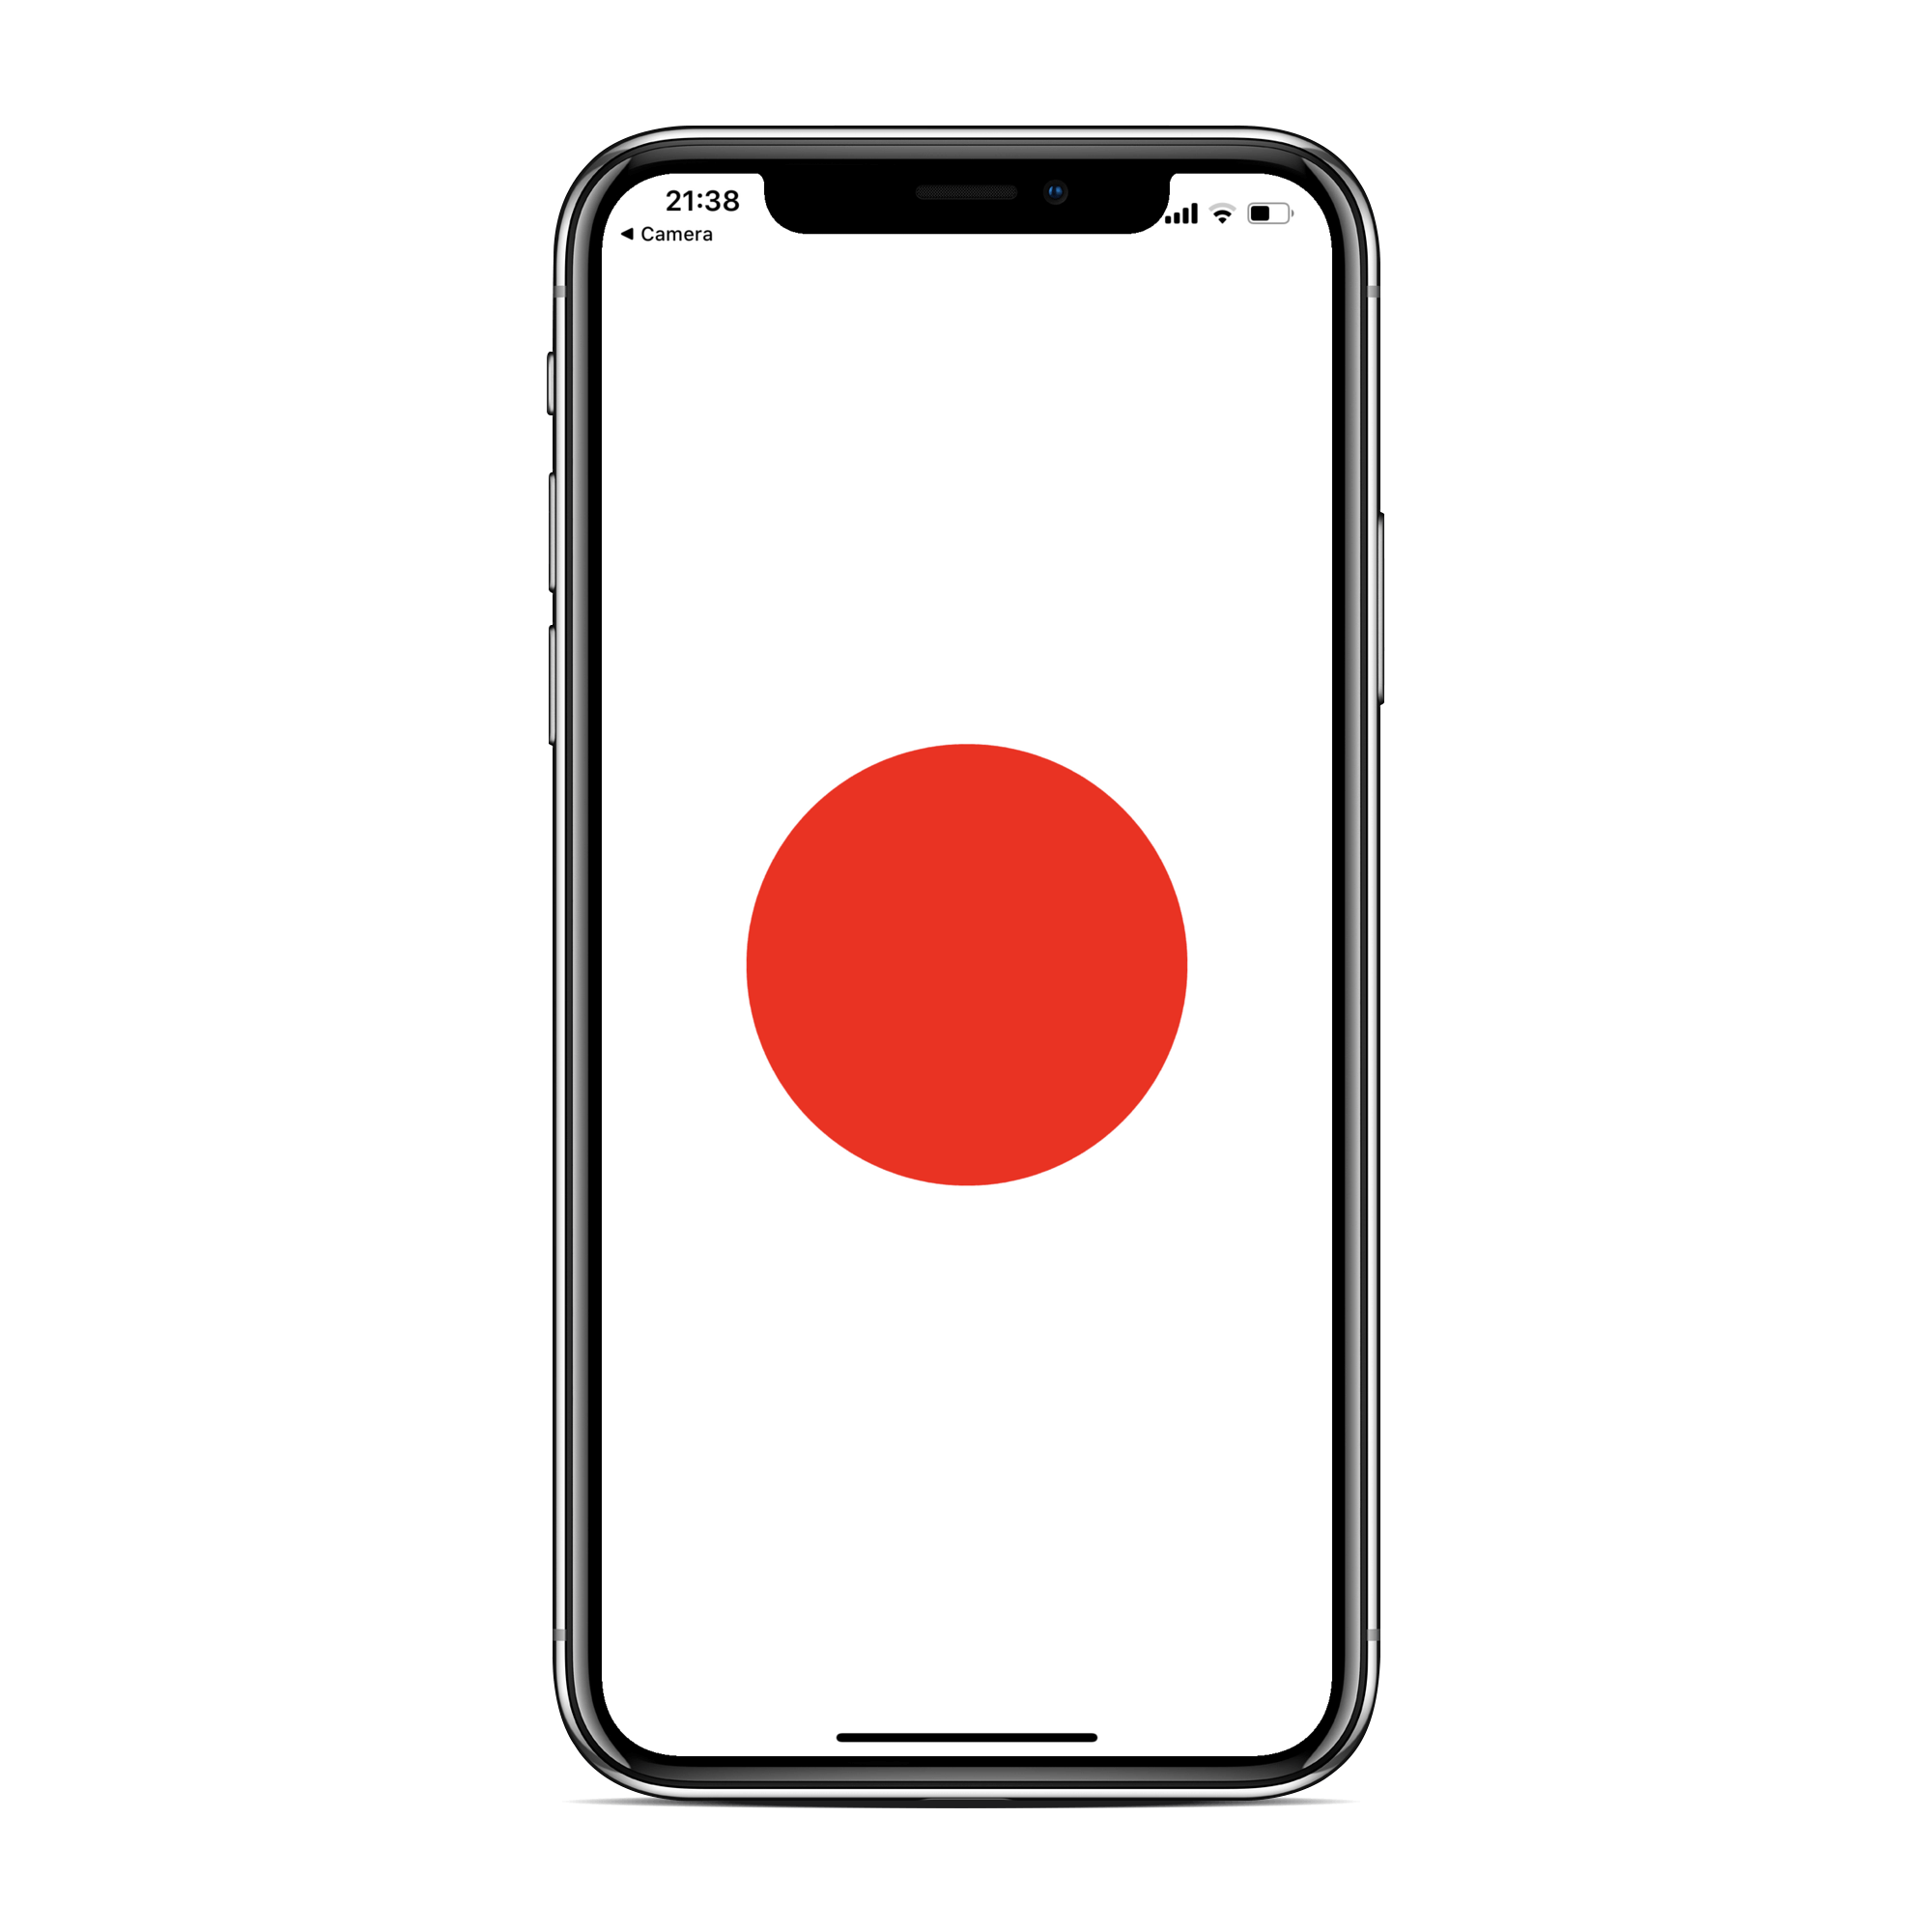
\includegraphics[width=0.25\textwidth]{max_kt1_images/image2.png} & 
            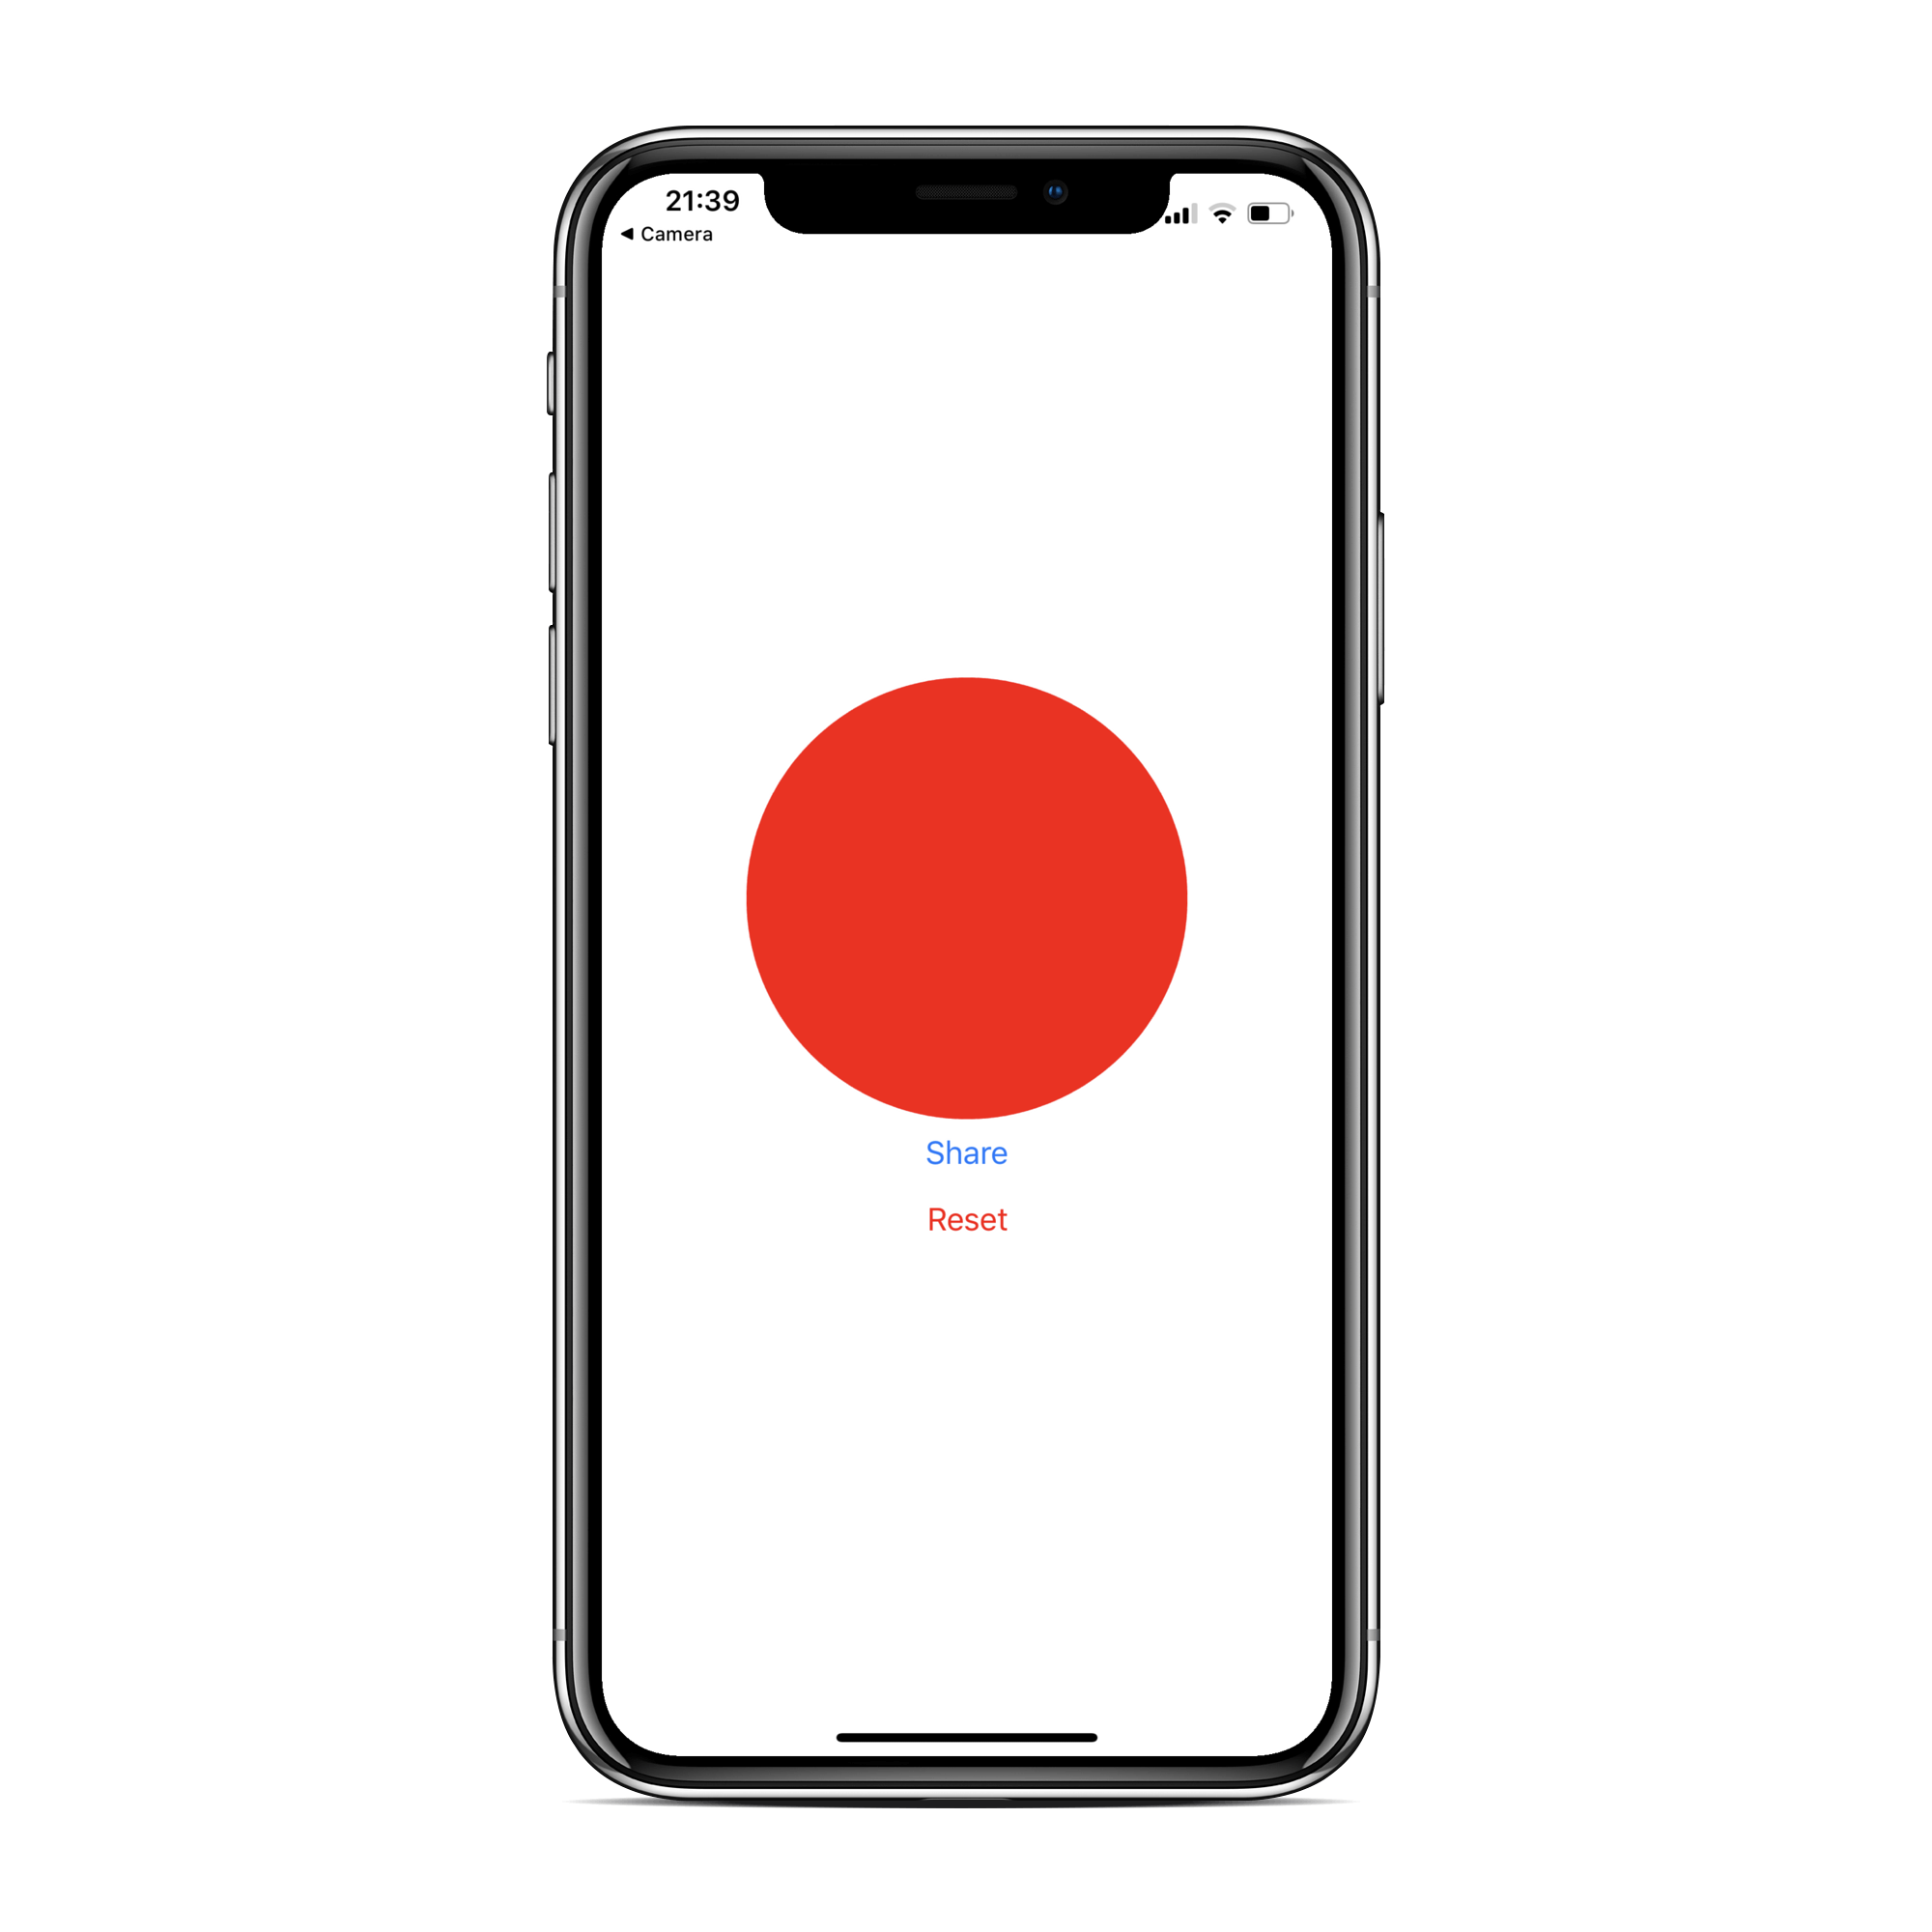
\includegraphics[width=0.25\textwidth]{max_kt1_images/image3.png} & 
            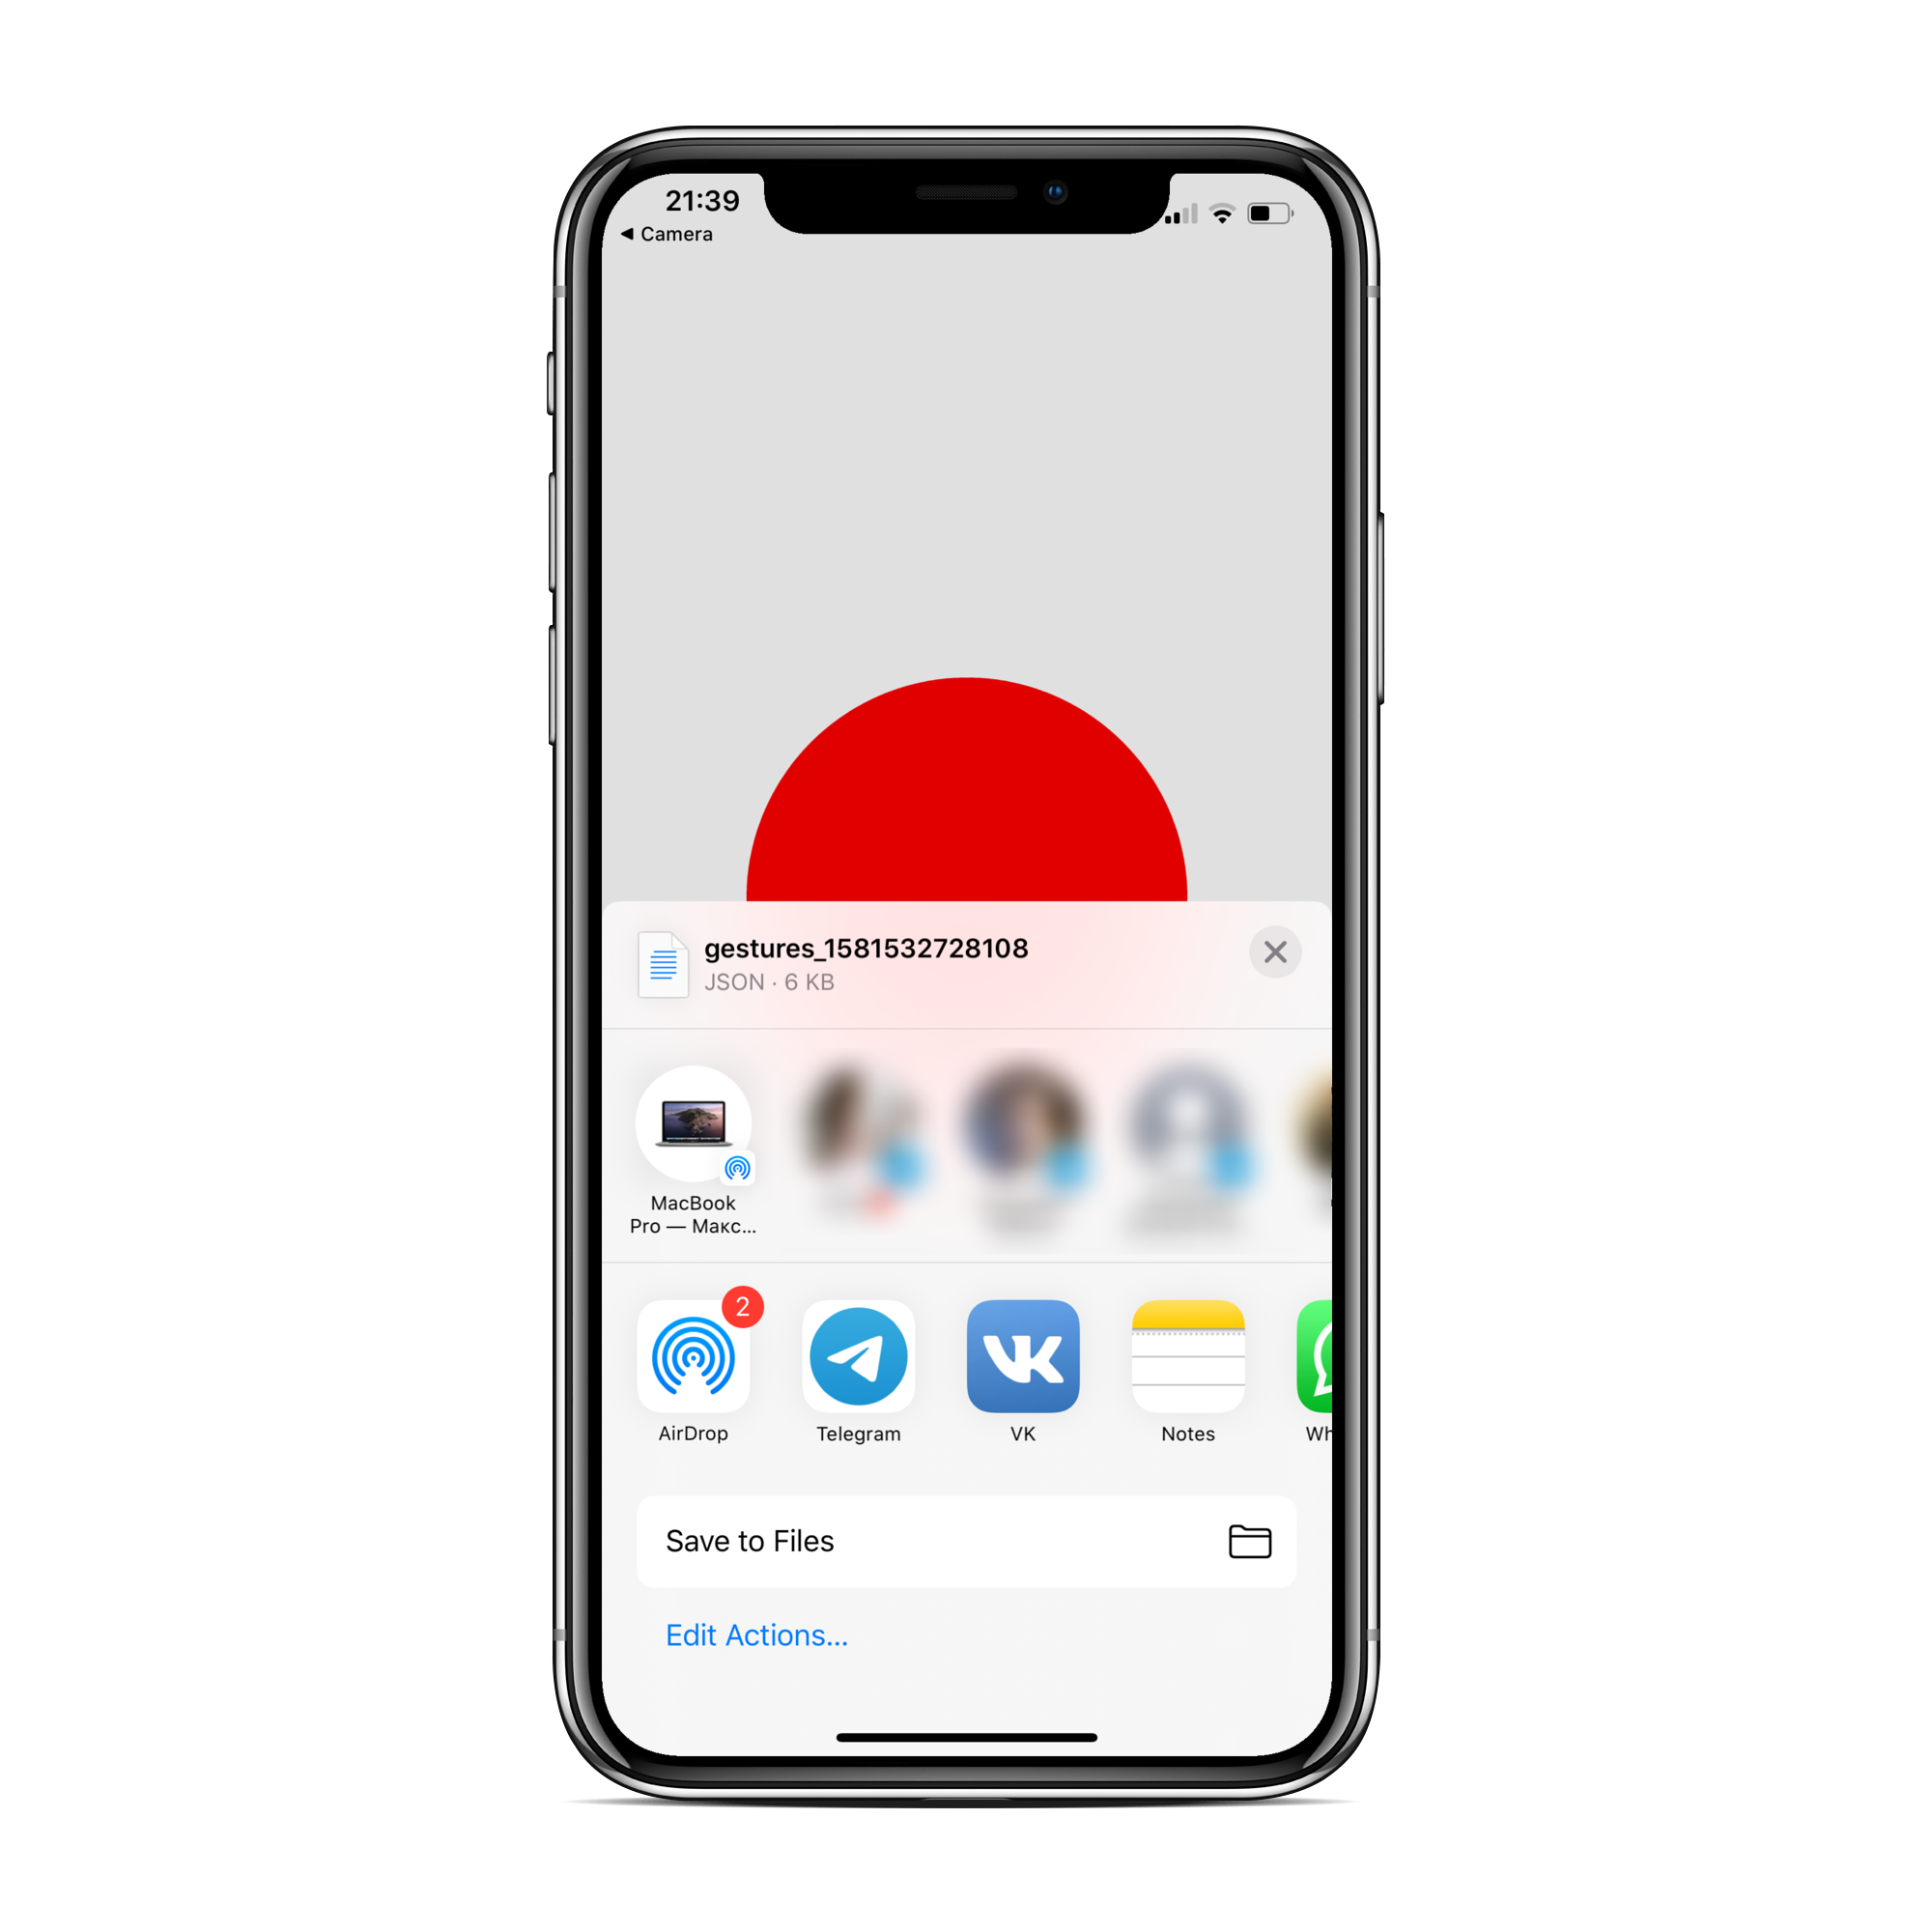
\includegraphics[width=0.25\textwidth]{max_kt1_images/image1.png} \\
        \end{tabular}
    \end{center}
    \caption{Интерфейс первой версии приложения.}
\end{figure}

% \subsection{КТ 2}

\subsubsection{Доработка приложения }
Далее, было необходимо доработать мобильное приложение. Хотелось бы видеть результат распознавания сразу после записи какого-либо жеста, для чего было решено сделать http сервер на node.js и доработать мобильное приложение так, чтобы оно отправляло записанное движение на данный сервер, а сервер в свою очередь запускал алгоритм распознавания и возвращал результат его работы обратно в приложение.
\begin{figure}[H]
    \begin{center}
        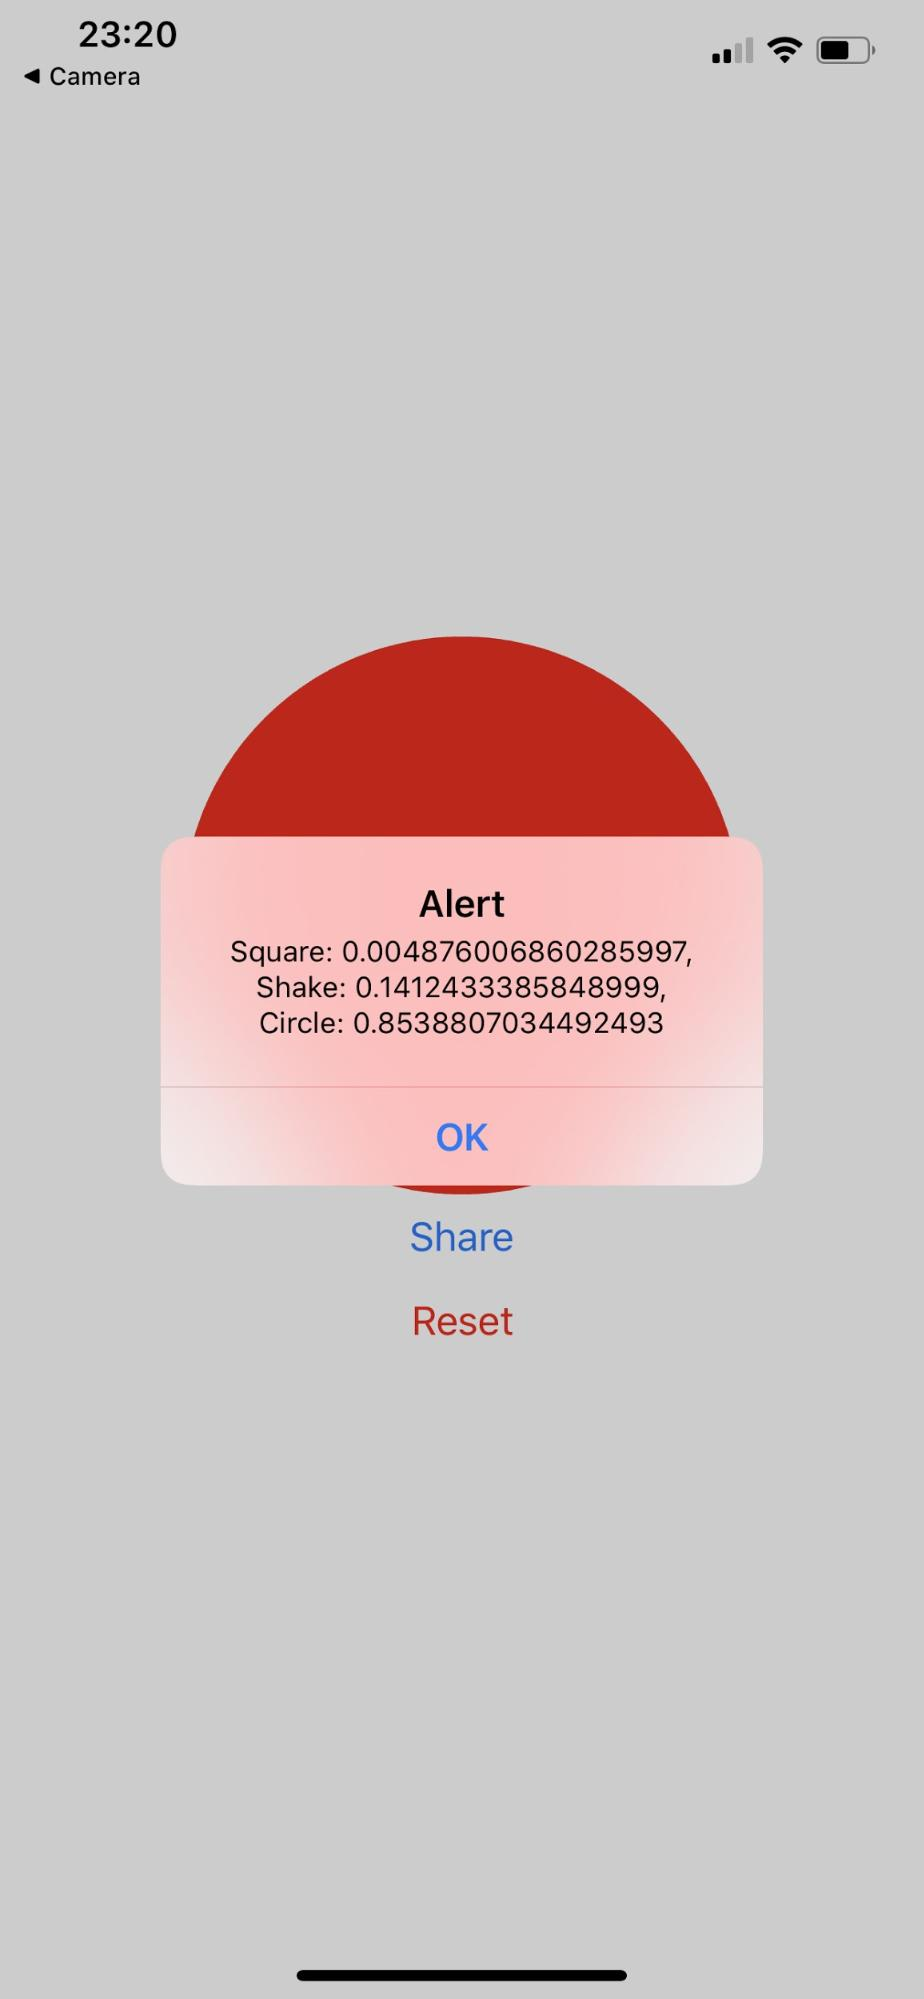
\includegraphics[width=0.2\textwidth]{max_kt2_images/image5.jpg}
    \end{center}
    \caption{Интерфейс усовершенствованного мобильного приложения. Снимок экрана был сделан сразу после записи движения.}
\end{figure}

\subsubsection{Последняя версия}
Затем, в связи с наличием практически полностью готовой библиотеки для обучения и распознавания жестов, разработанной одним из участников нашей команды, было решено все-таки переделать приложение, чтобы повысить удобство его использования. Пришлось практически полностью переработать интерфейс. Теперь приложение имеет две вкладки: тренировка и распознавание. Они отвечают, как следует из названия, за тренировку и распознавание соответственно.

Тестирование происходит следующим образом: зажимается кнопка \textit{Record} и выполняется движение. Далее приложение, используя программную библиотеку, получает результат распознавания. В результате чего на экране появляется изображение восстановленного жеста и предсказание алгоритма в виде надписи вида \textit{"I guess it's a <название жеста>"}. Далее, при желании можно нажать на кнопку \textit{Reset}, чтобы записать новый жест.
\begin{figure}[H]
    \begin{center}
        \begin{tabular}{ccc}
            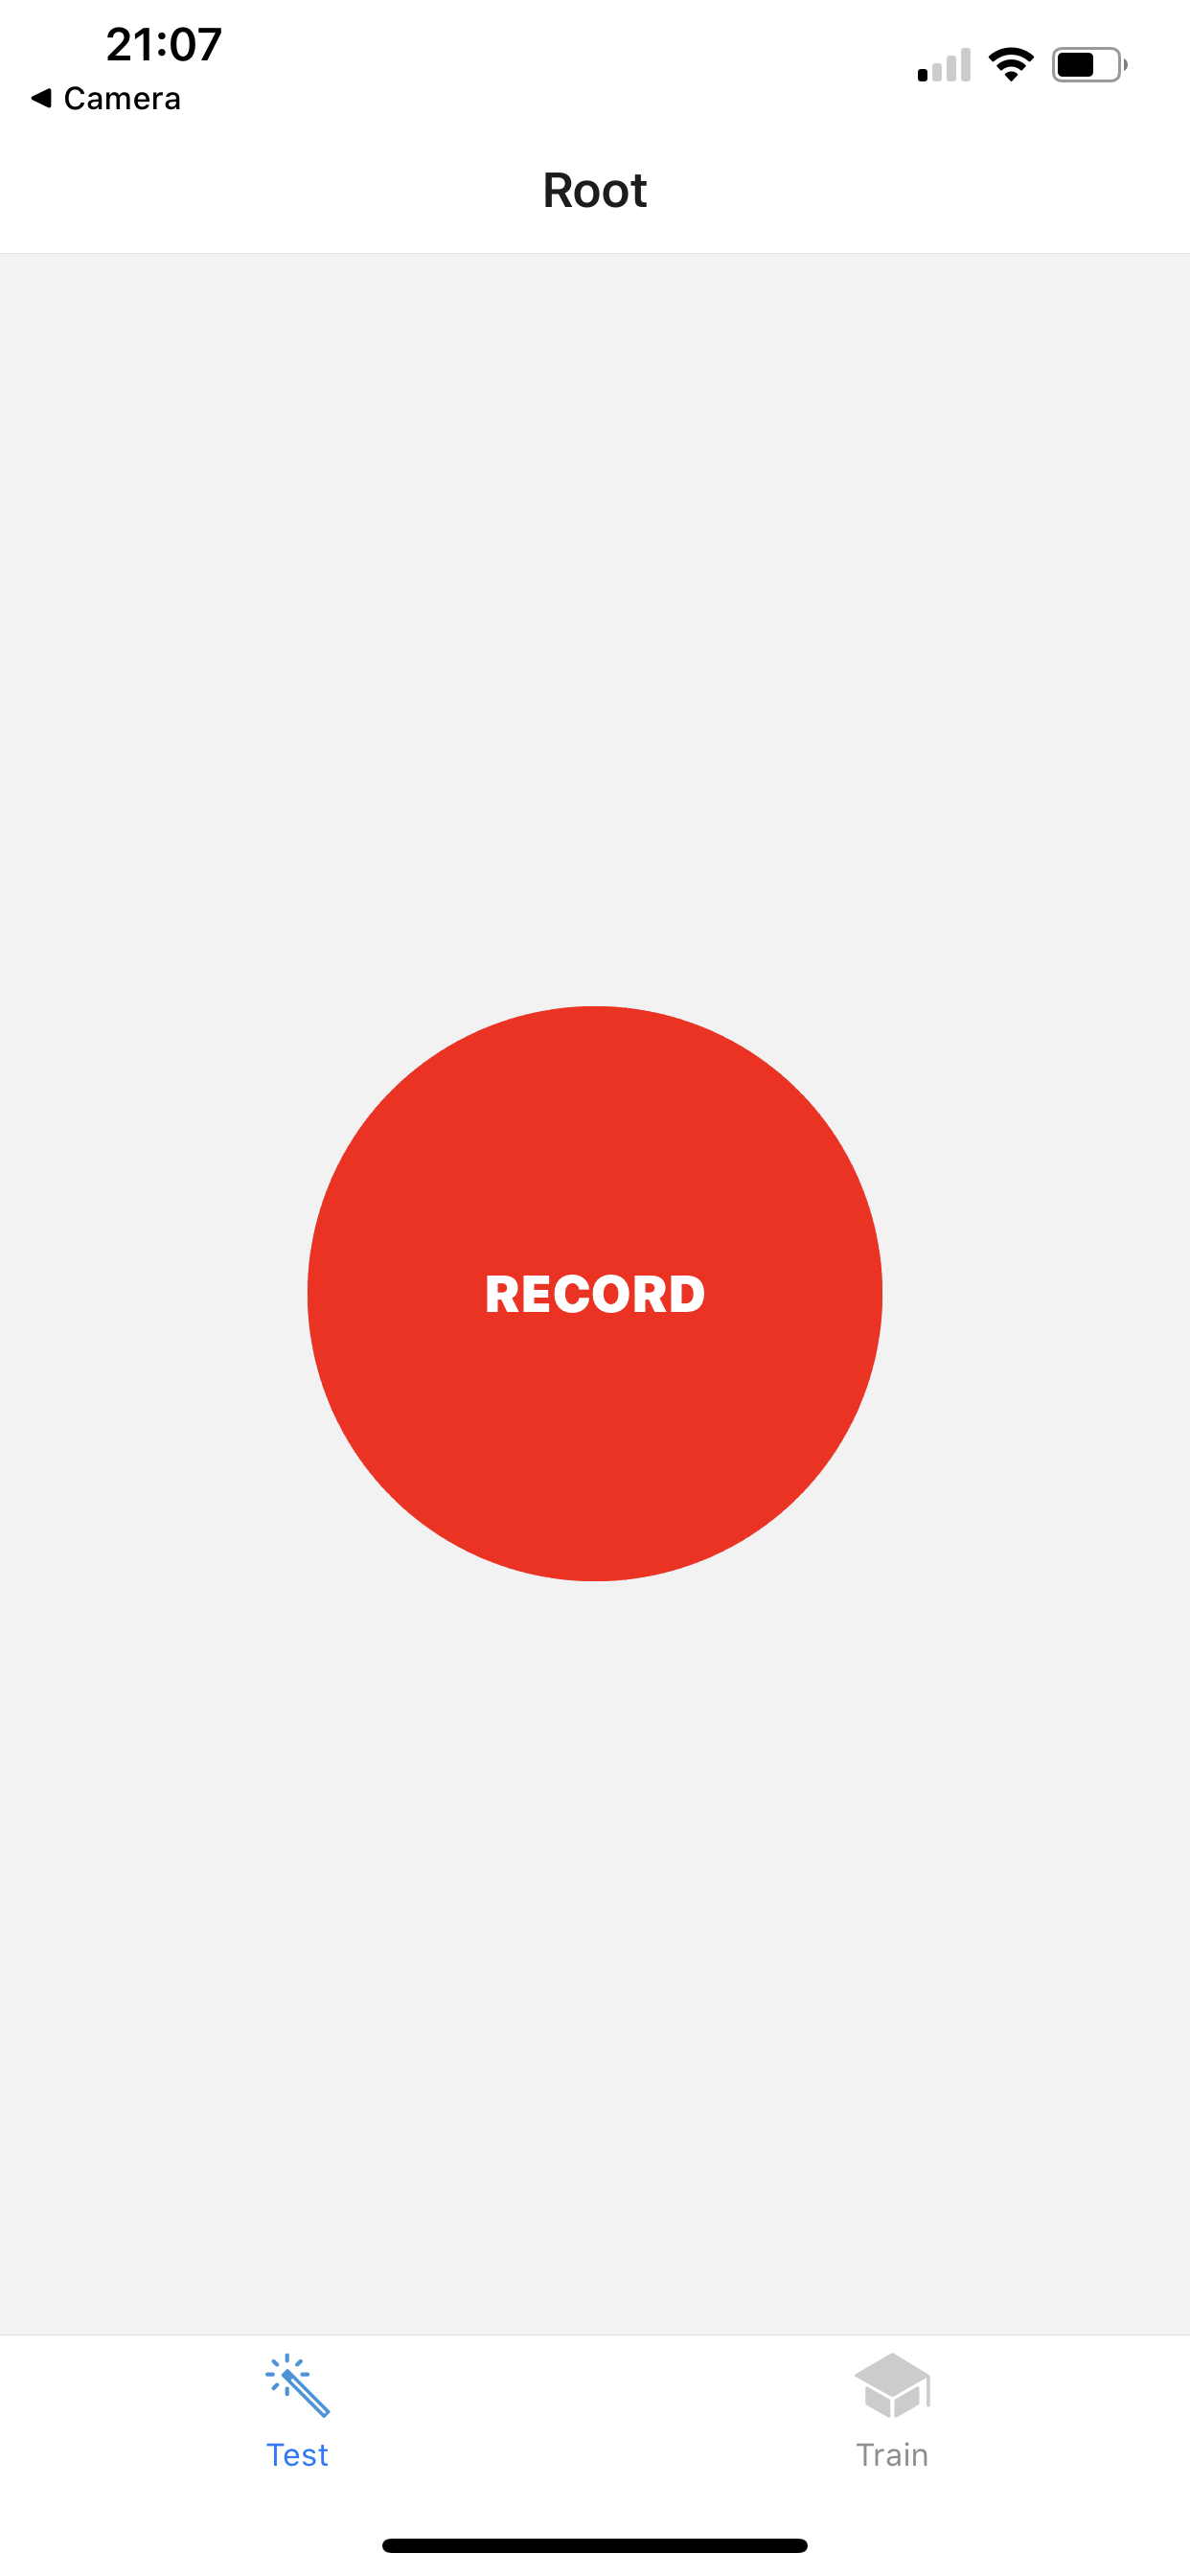
\includegraphics[width=0.15\textwidth]{testingapp_screenshots/IMG_2011.PNG} & 
            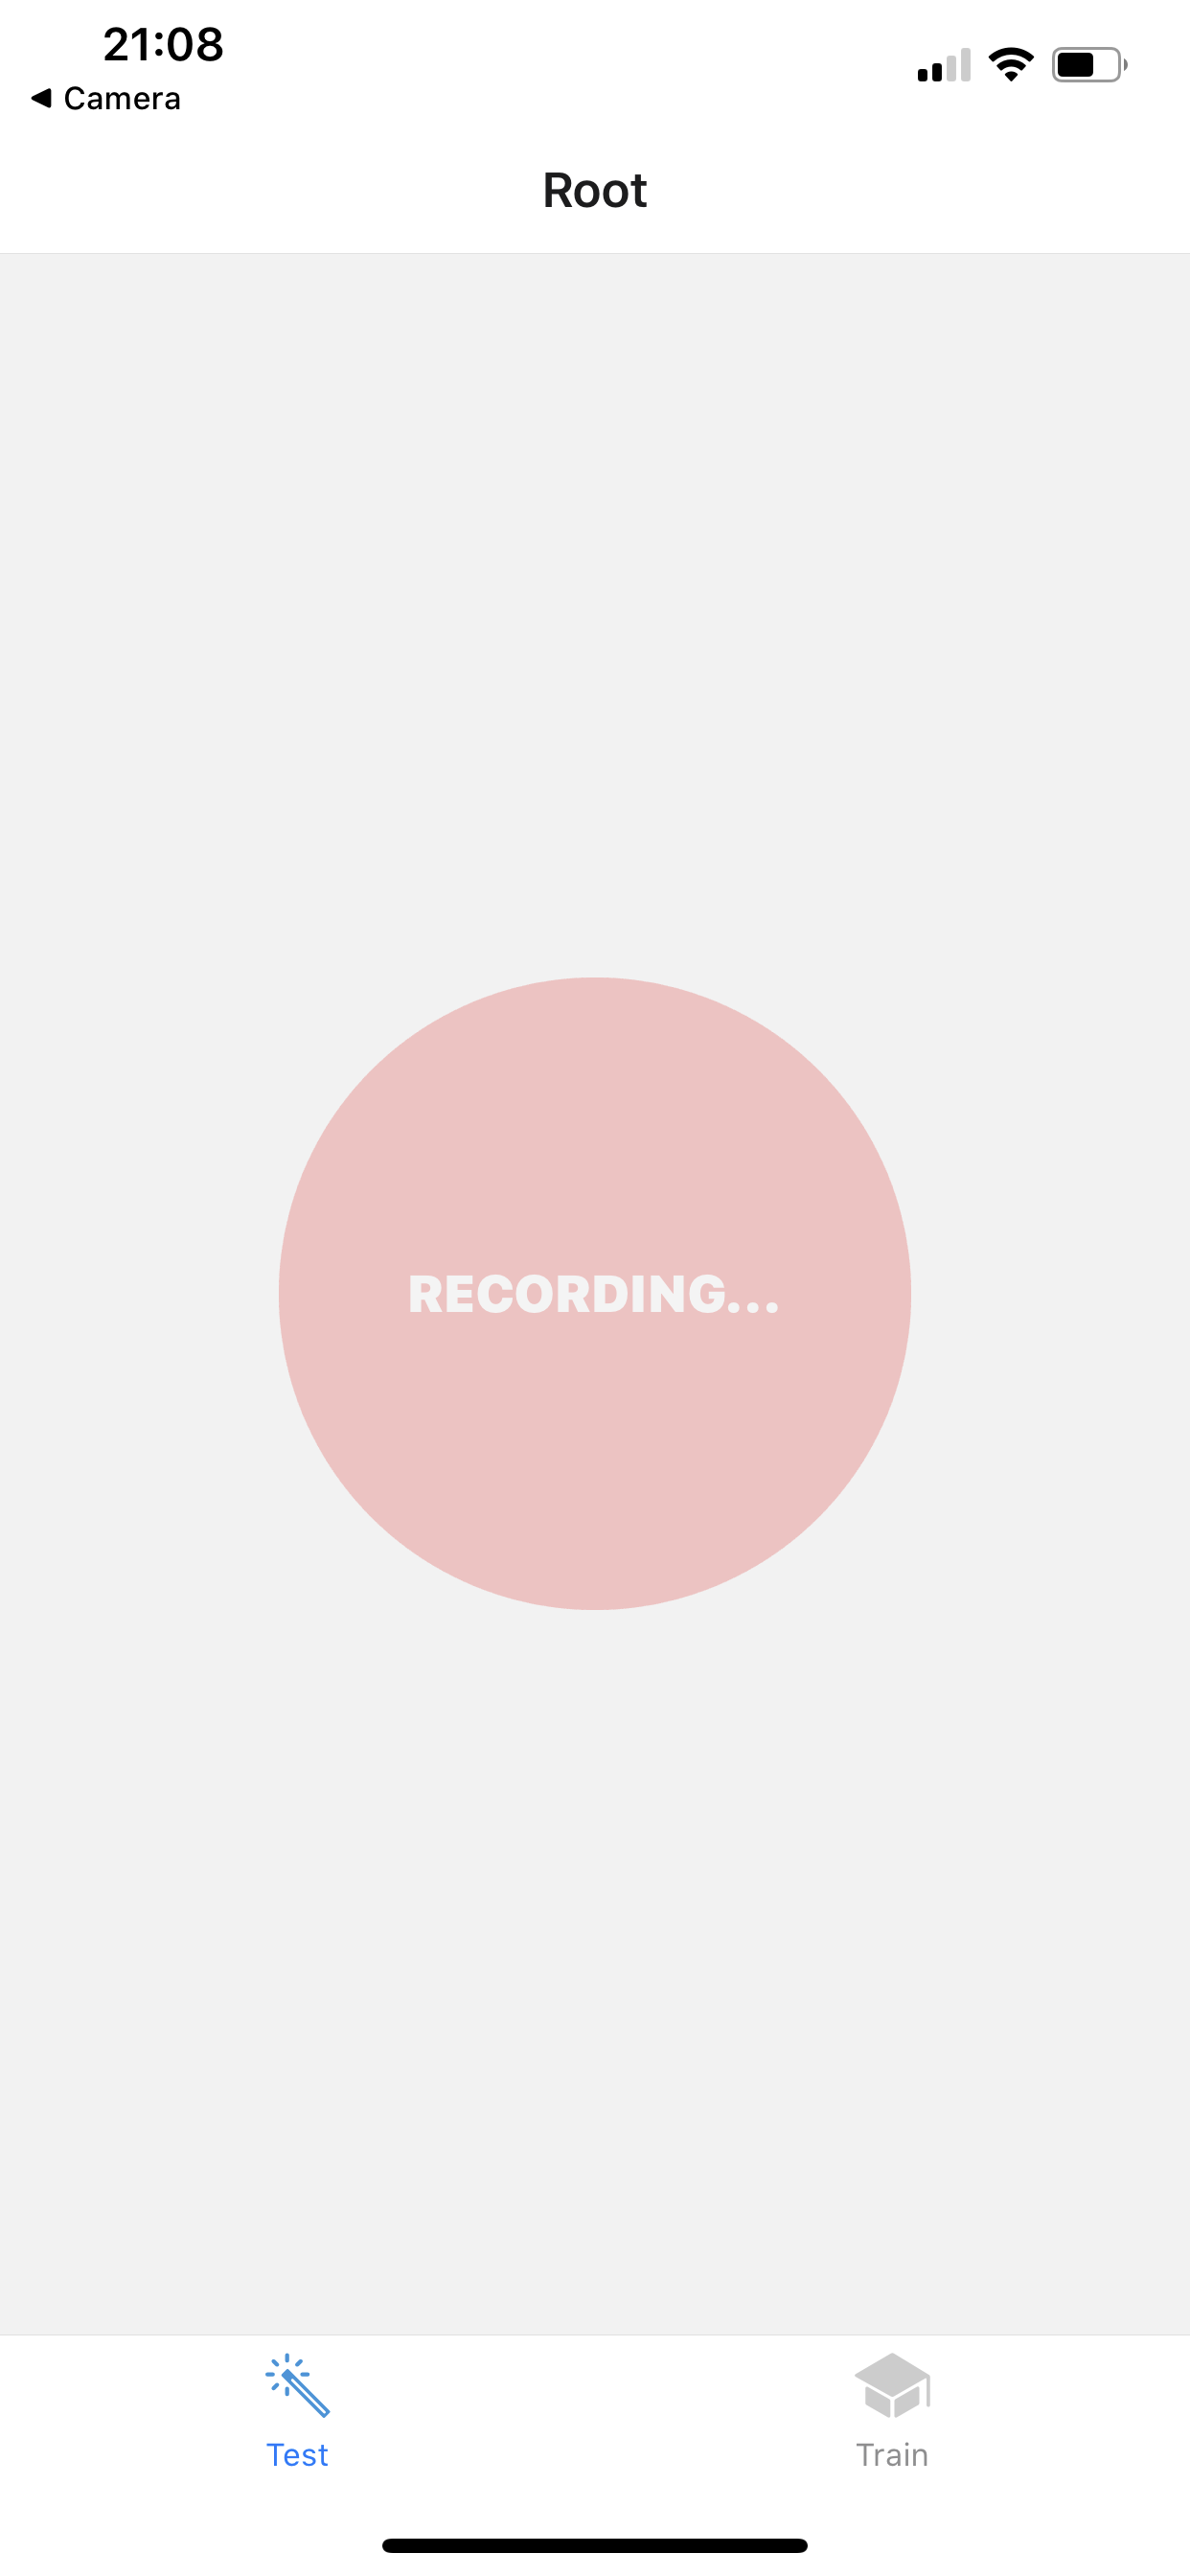
\includegraphics[width=0.15\textwidth]{testingapp_screenshots/IMG_2016.PNG} & 
            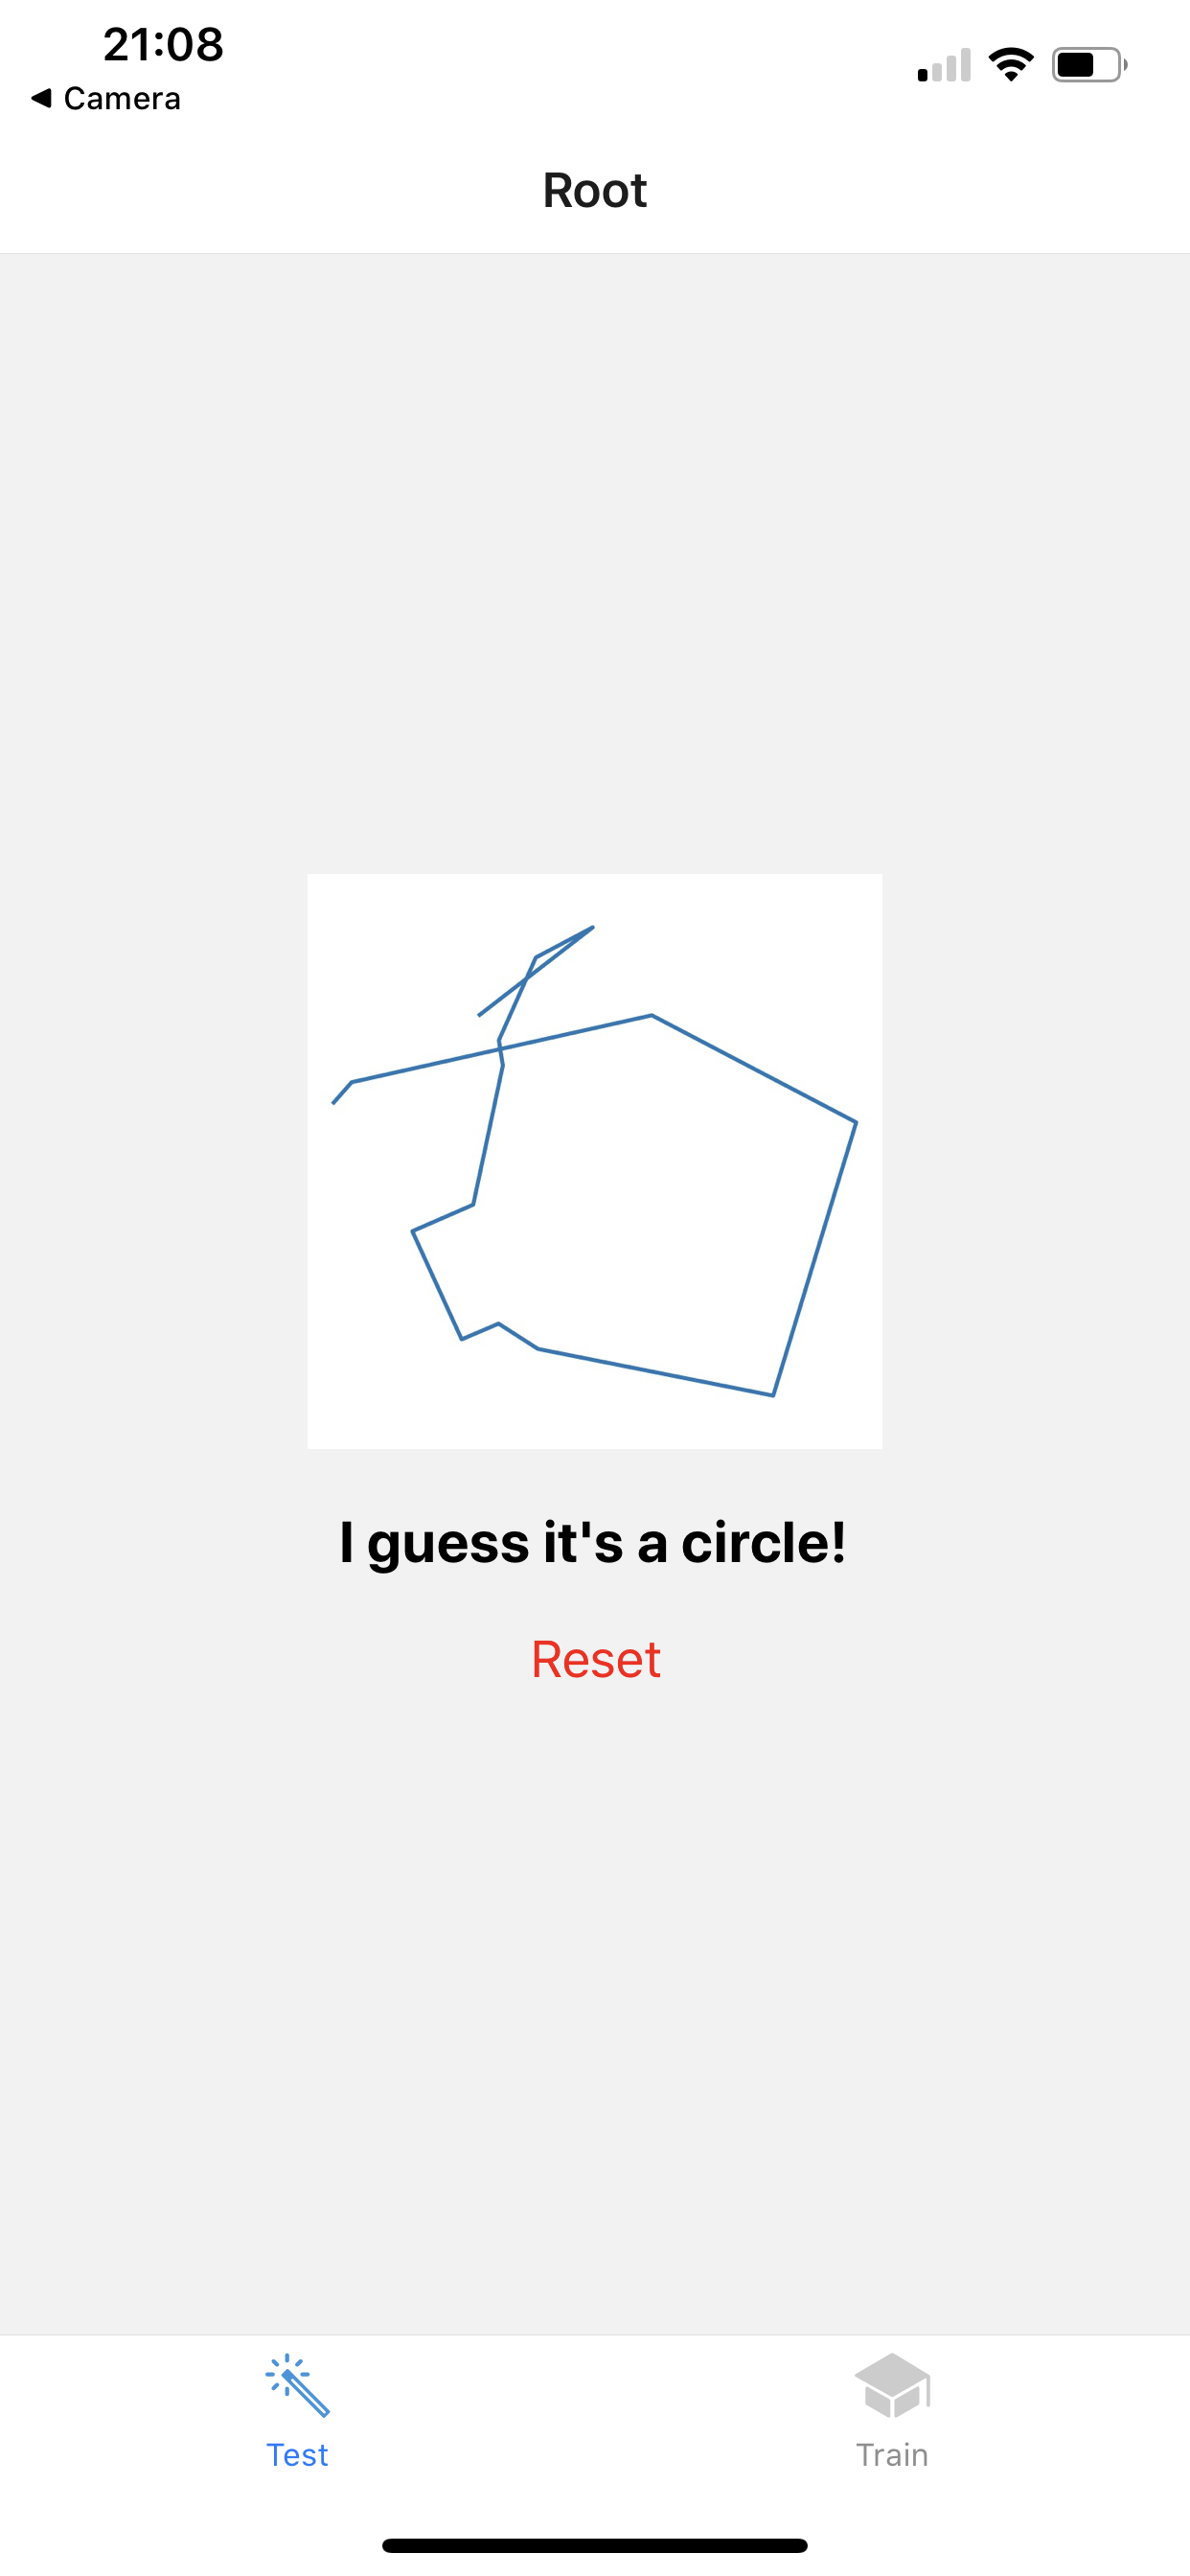
\includegraphics[width=0.15\textwidth]{testingapp_screenshots/IMG_2017.PNG} \\
        \end{tabular}
    \end{center}
    \caption{Интерфейс тестирования в различных состояниях.}
\end{figure}

Процесс обучения немного отличается: жест записывается аналогичным образом, но после записи жеста появляются 3 кнопки: \textit{Reset, Submit} и \textit{Share}. Первая кнопка работает тем же образом, что и при тестировании, третья отвечает за отправку записанного жеста с помощью AirDrop, Telegram, электронной почты и т.д. При нажатии на кнопку \textit{Submit} записанные данные с помощью программной библиотеки отправляются на сервер, а он в свою очередь возвращает изображение жеста восстановленное из этих данных. Затем, оно появляется на месте кнопки записи жеста.
\begin{figure}[H]
    \begin{center}
        \begin{tabular}{cccc}
            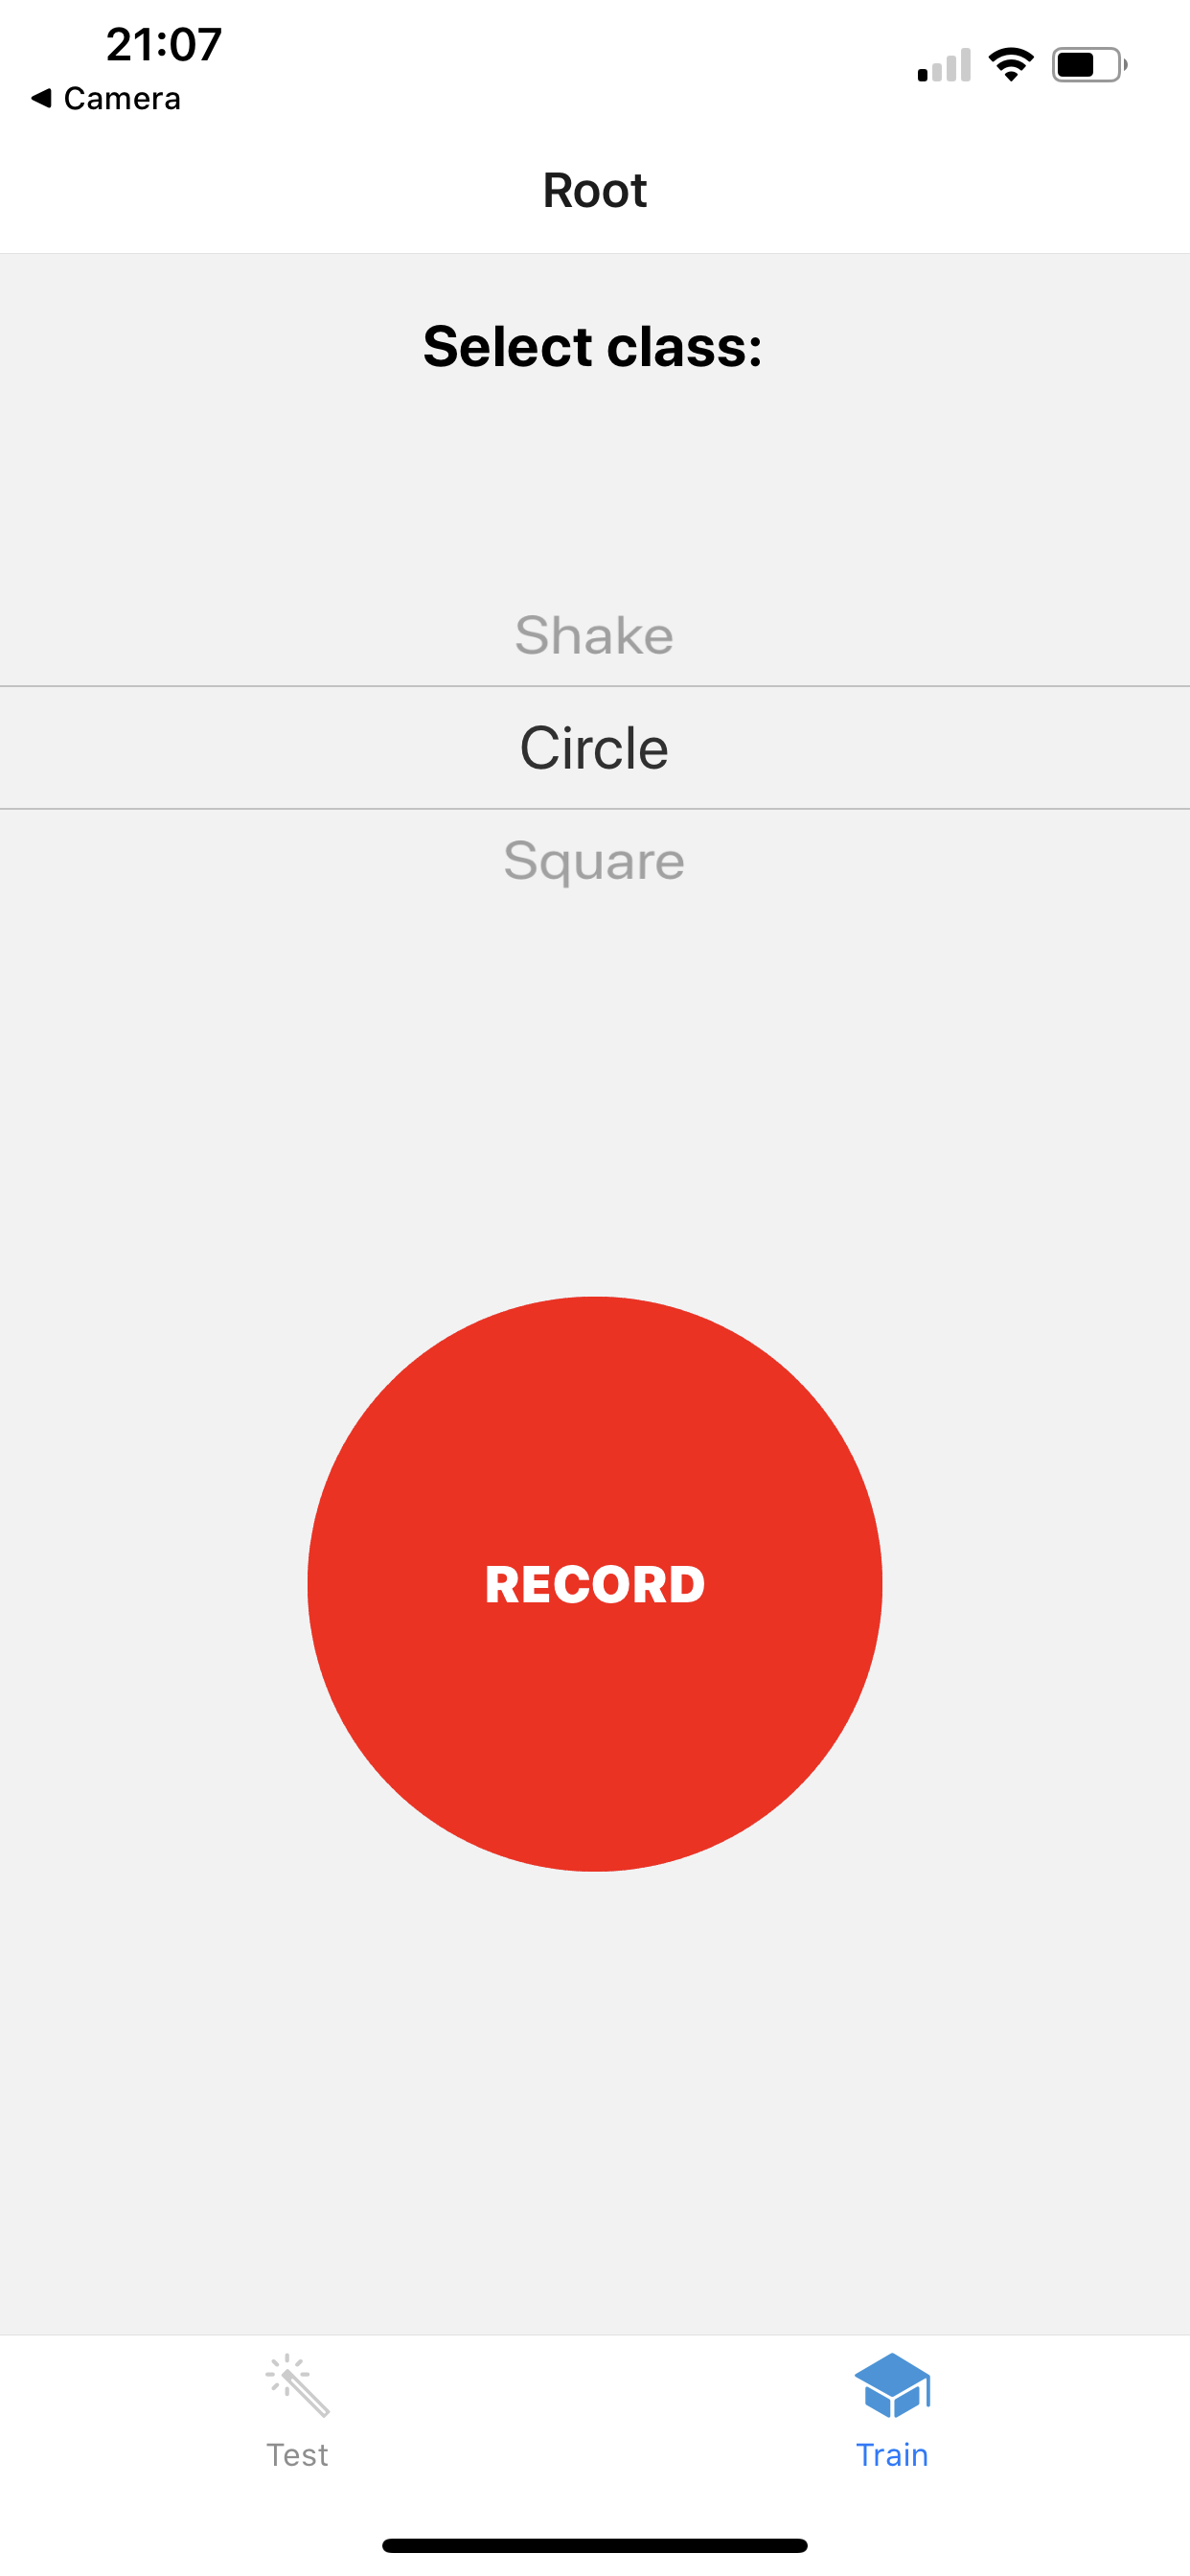
\includegraphics[width=0.15\textwidth]{testingapp_screenshots/IMG_2012.PNG} & 
            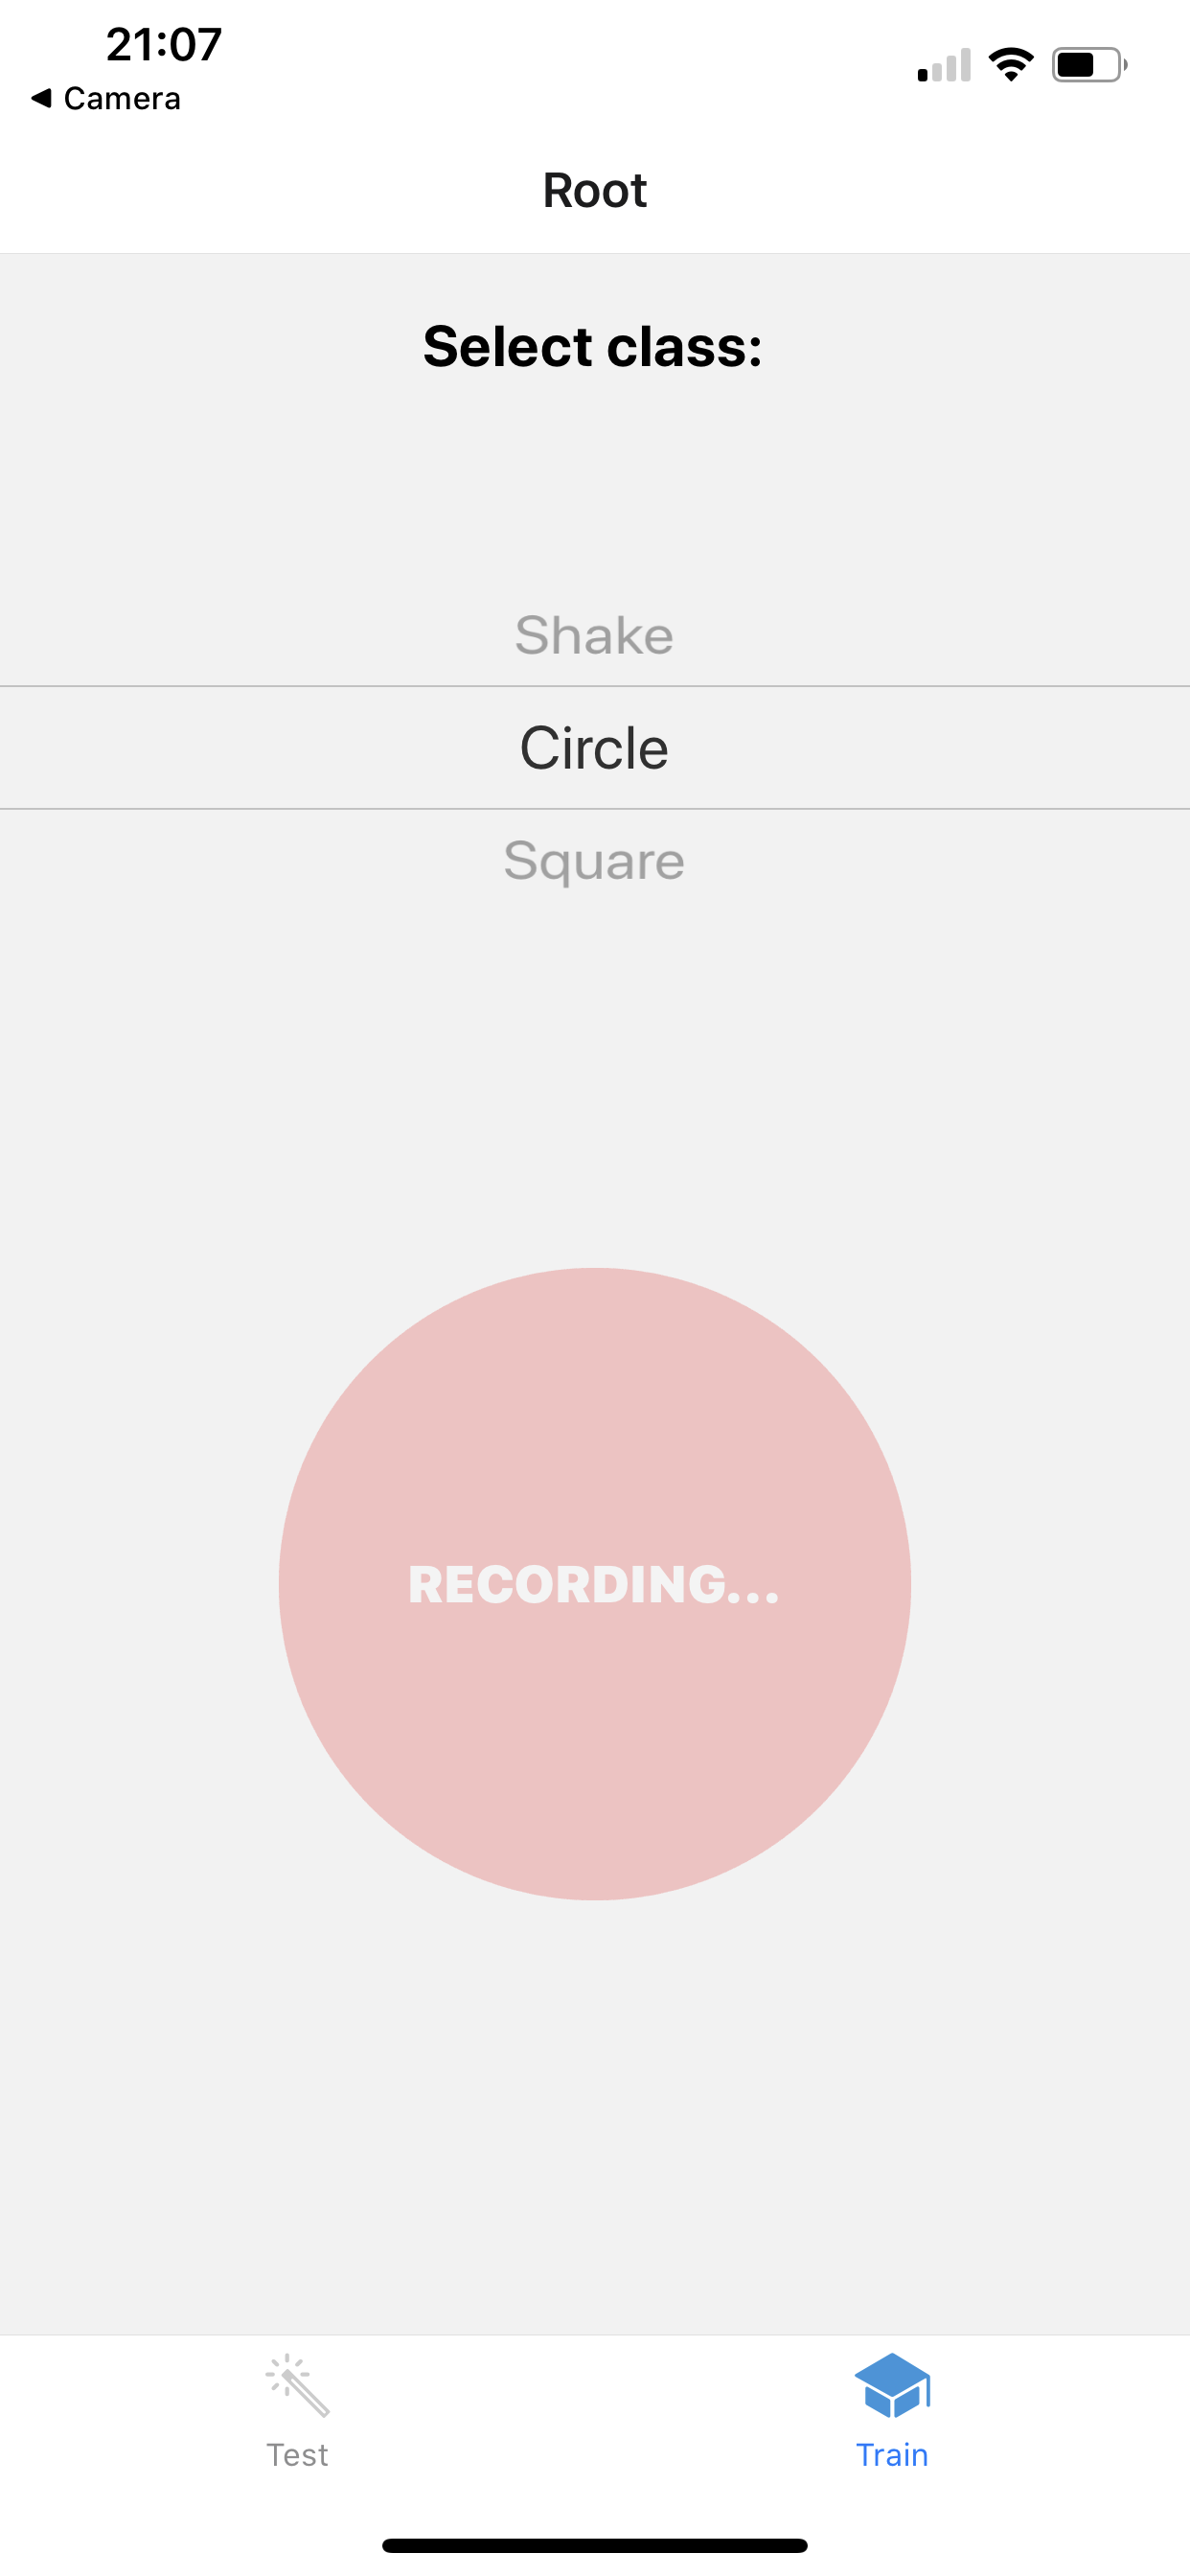
\includegraphics[width=0.15\textwidth]{testingapp_screenshots/IMG_2013.PNG} & 
            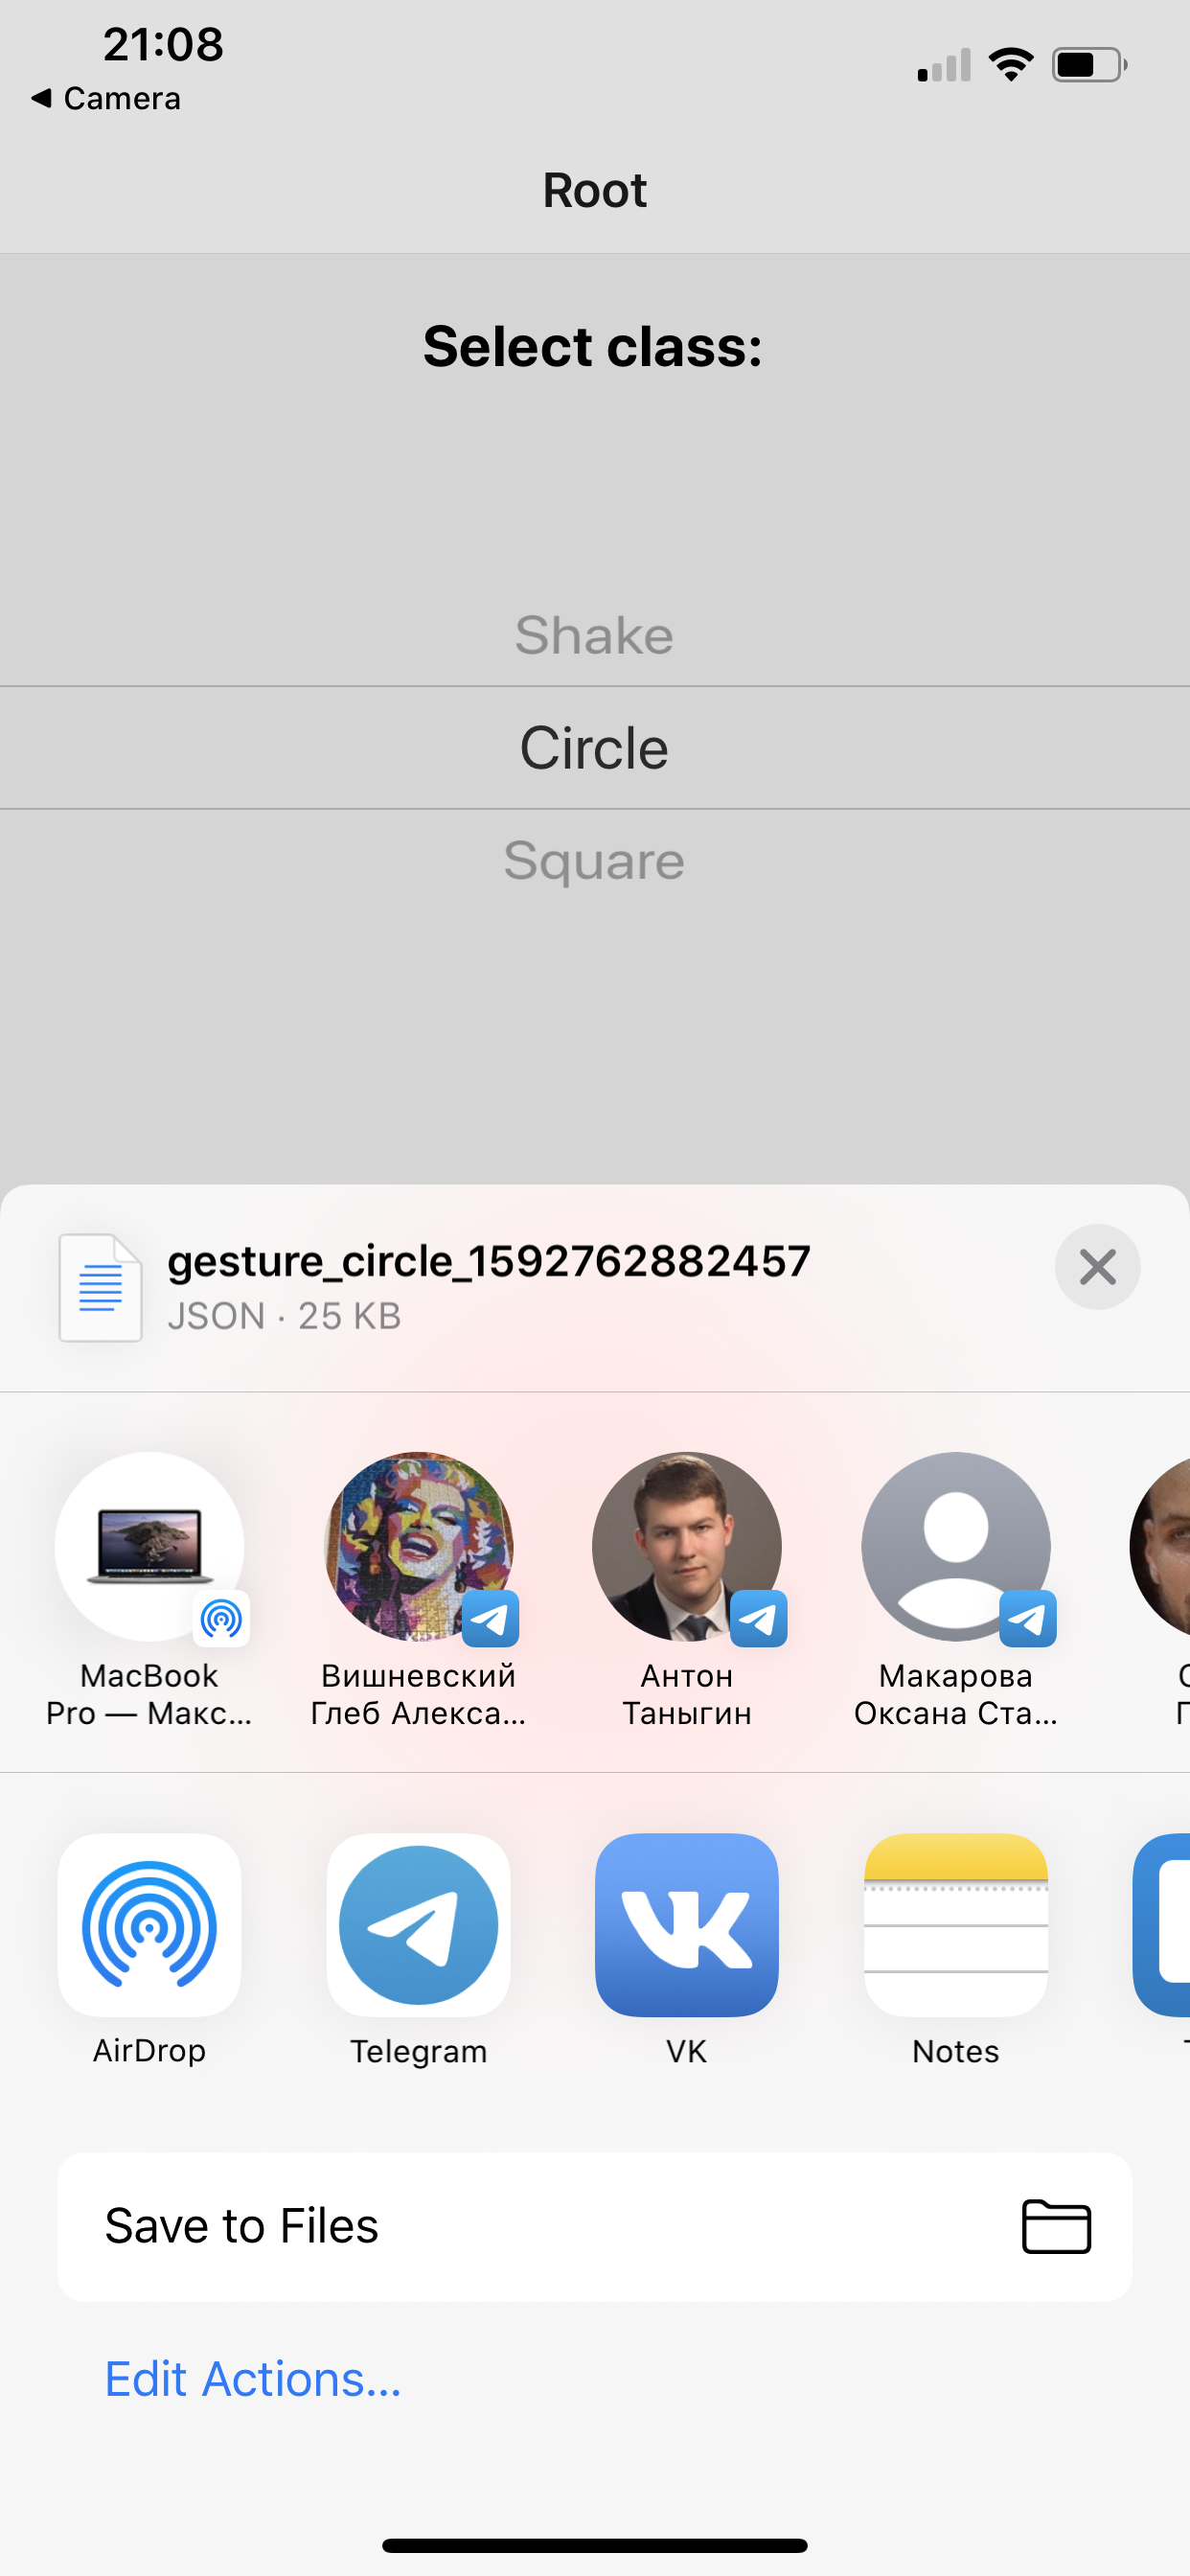
\includegraphics[width=0.15\textwidth]{testingapp_screenshots/IMG_2014.PNG} & 
            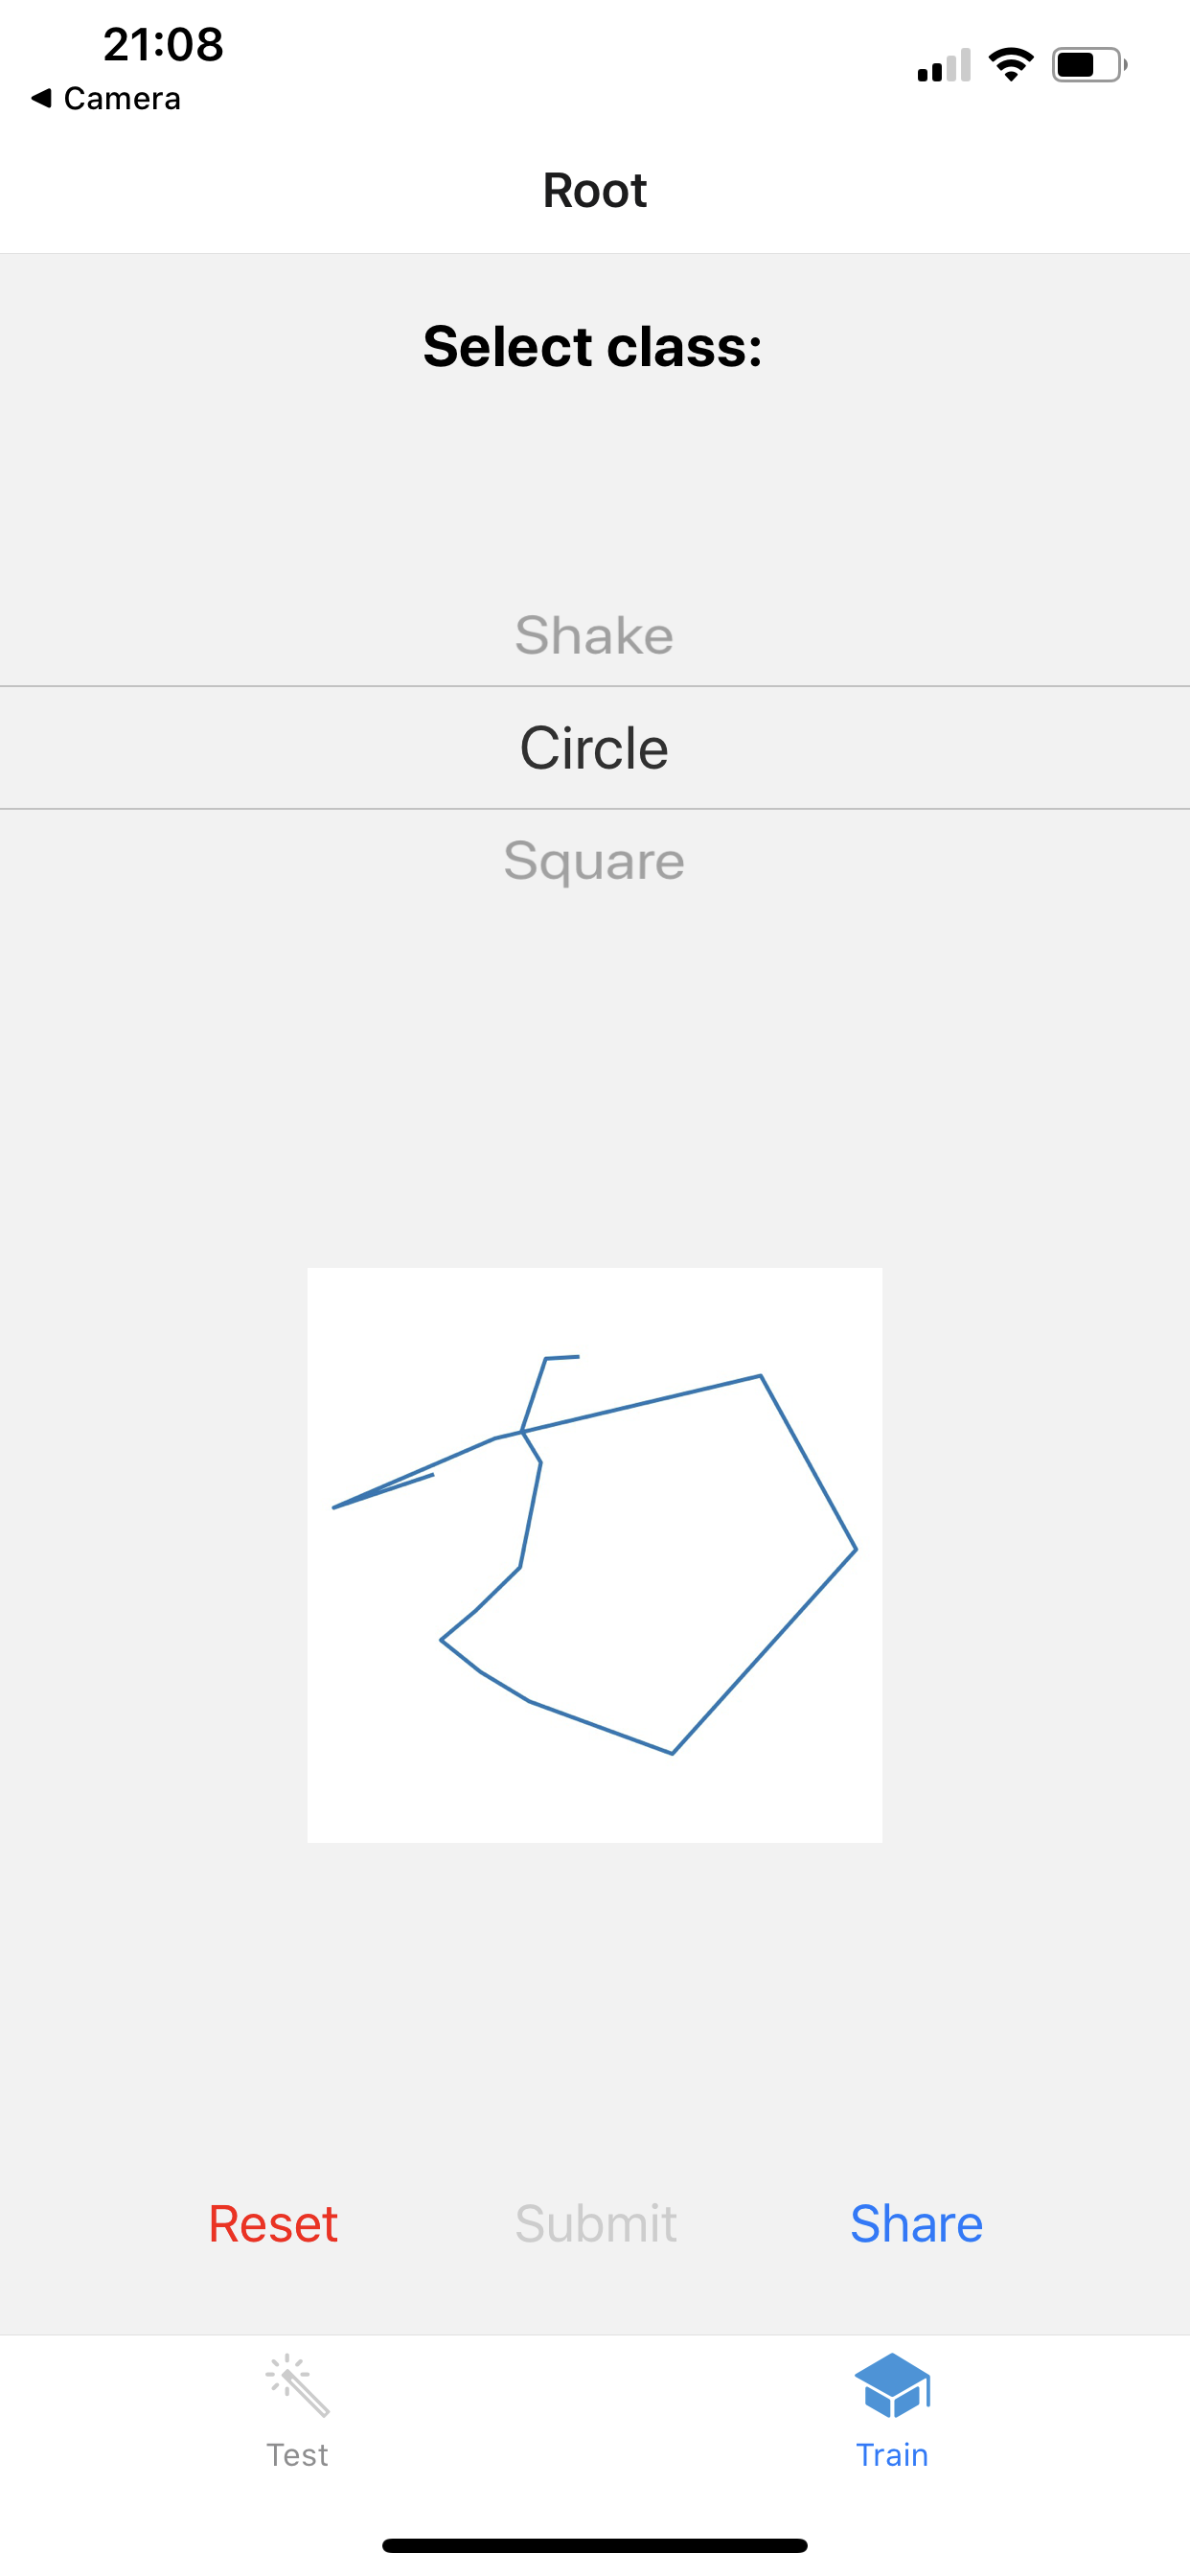
\includegraphics[width=0.15\textwidth]{testingapp_screenshots/IMG_2015.PNG} \\
        \end{tabular}
    \end{center}
    \caption{Интерфейс обучения в различных состояниях.}
\end{figure}